\documentclass[10pt, uplatex, dvipdfmx]{jsarticle}
\usepackage{amsmath,amsthm,amssymb,amsfonts,enumerate, braket,
  setspace, bm, multirow, ascmac, graphicx, emathEy, docmute, url,
  ulem, wrapfig}


\makeatletter
\renewenvironment{proof}[1][\proofname]{\par
  \pushQED{\qed}%
  \normalfont \topsep6\p@\@plus6\p@\relax
  \trivlist
  \item\relax
  {\bfseries
  #1\@addpunct{.}}\hspace\labelsep\ignorespaces
}{%
  \popQED\endtrivlist\@endpefalse
}
\makeatother

\pagestyle{plain}

\theoremstyle{definition}
\newtheorem{theorem}{定理}[section]
\newtheorem*{theorem*}{定理}
\newtheorem*{definition}{定義}
\newtheorem{lemma}[theorem]{補題}
\newtheorem{example}[theorem]{例}
\newtheorem*{example*}{例}
\newtheorem*{remark}{注意}
\newtheorem*{promis}{約束}
\renewcommand{\proofname}{\textbf{証明}}

\newtheorem*{fundamental}{\textbf{微分積分学の基本定理}}

\numberwithin{equation}{section}


\newcommand{\ds}{\displaystyle}




\title{\Huge 数学II / 2}
\author{\Large 内海 和樹}

\begin{document}


\maketitle

\begin{center}
  「3 分数関数の積分」まで
\end{center}

\vspace{5zh}
\begin{center}
  {\LARGE 積分基本問題集}

  \begin{itemize}
    \setlength{\itemsep}{2zh}
    
  \item 壱(1変数) \url{https://github.com/kazutsumi/Integral1/blob/main/integral1.pdf}
    \begin{figure}[h]
      \centering
      \includegraphics[width=3cm]{./pictures/QR/1.png}
    \end{figure}
    
  \item 弍(2変数) \url{https://github.com/kazutsumi/Integral2/blob/main/integral2.pdf}
    \begin{figure}[h]
      \centering
      \includegraphics[width=3cm]{./pictures/QR/2.png}
    \end{figure}
  \end{itemize}
\end{center}


\thispagestyle{empty}

\clearpage

\tableofcontents

\newpage

目次ページが続く

\newpage

まだ目次ページ

\newpage

たぶんここまで目次ページ

\newpage

\section{不定積分計算の基礎}

\subsection{基礎中の基礎}\label{subsec:fundamental}

なにはともあれ,以下の微分公式を思い出しておこう.いずれも春学期に学んだはず.
\[\renewcommand{\arraystretch}{1.3}
  \begin{array}[h]{c|ccccccccc}
    f(x) & x^n & e^x & \log|x| & \sin x & \cos x & \tan x & \sin^{-1}x & \cos ^{-1} x & \tan^{-1} x\\ \hline
    \\
    f'(x) & n x^{n-1} & e^x & \dfrac{1}{x} & \cos x & -\sin x & \dfrac{1}{\cos^2x} & \dfrac{1}{\sqrt{1-x^2}}
                                                                       & -\dfrac{1}{\sqrt{1-x^2}} & \dfrac{1}{1+x^2}
  \end{array}
\]
この表を逆に読むことで,以下の基礎中の基礎の公式を導ける.面倒なので,以降積分定数は省略する.

\vspace{1zh}

\begin{itemize}
  \setlength{\itemsep}{2zh}
  
\item
  $\ds x^n = \frac{n+1}{n+1}~\!x^n = \frac{1}{n+1}\left(
    x^{n+1}\right)' = \left( \frac{1}{n+1}~\!
    x^{n+1}\right)'$ より \fbox{\;
    $\ds \int x^n \ dx = \frac{1}{n+1}~ \! x^{n+1}  \quad (n \neq -1)$\;}

\item $e^x = \left( e^x \right) ' $ より \fbox{ \; $\ds \int e^x \ dx = e^x $ \; }

\item $\ds \frac{1}{x} = \left( \log x \right)' $ より \fbox{ \; $\ds \int \frac{dx}{x} = \log x $ \; }

\item $\ds \cos x = \left( \sin x \right)'$ より \fbox{ \; $\ds \int \cos x \ dx = \sin x $ \; }

\item
  $\ds \sin x = - \left( - \sin x \right) = - \left( \cos x\right)' =
  \left(- \cos x \right)'$ より \fbox{\;
    $\ds \int \sin x \ dx = -\cos x $ \; }

\item $\ds \frac{1}{\cos^2 x} = \left( \tan x \right)'$ より \fbox{\; $\ds \int \frac{dx}{\cos^2 x} = \tan x $\;}

\item $\ds \frac{1}{\sqrt{1-x^2}} = \left( \sin^{-1}x
  \right)'$ より \fbox{\;
    $\ds \int \frac{dx}{\sqrt{1-x^2}} = \sin^{-1}x $\;}

\item
  $\ds \frac{1}{\sqrt{1-x^2}} = - \left(
    -\frac{1}{\sqrt{1-x^2}}\right) = - \left( \cos^{-1} x \right)' =
  \left( -\cos^{-1}x \right)'$ より \fbox{ \;
    $\ds \int \frac{dx}{\sqrt{1-x^2}} = -\cos^{-1} x $\;}

 \item $\ds \frac{1}{1+x^2} = \left( \tan^{-1}x\right)'$ より \fbox{\;  $\ds \int\frac{dx}{1+x^2} = \tan^{-1} x $ \;}
\end{itemize}

\newpage

初めの公式 $\ds \int x^n \ dx = \frac{1}{n+1}~\! x^{n+1} $ において $n$ は自然数だけでなく,
\[
  \int \frac{1}{x^2} \ dx = \int x^{-2} \ dx = -x^{-1},\qquad
  \int \sqrt{x} \ dx = \int
  x^{\frac{1}{2}} \ dx =\frac{2}{3} x^{\frac{3}{2}}
\]
のように,$n=-2$ や $n=1/2$ などでも適用できるので,結構適用範囲が広い.\\


合成関数の微分公式から,例えば $\left( \sin\left(3x\right)\right)' = 3
\cos(3x)$
なので,$\ds \cos(3x) = \frac{1}{3}\left( \sin (3x)\right)' = \left(
  \frac{1}{3} \sin(3x) \right)'$ である.これを逆に読んで
\[
 \int\cos (3x) \ dx = \frac{1}{3} \sin (3x)
\]
を導ける.他にも,例えば $\left( e^{-2x}\right)' = -2 e^{-2x}$ なの
で,$\ds e^{-2x} = -\frac{1}{2} \left( e^{-2x}\right)' = \left(
-\frac{1}{2} e^{-2x}\right)'$ より
\[
  \int e^{-2x} \ dx = -\frac{1}{2} e^{-2x}
\]
である.このように,どんな方法であれ関数 $f$ に対して $F' = f$ となる $F$ を見つけてしまえば
\[
  \int f(x) \ dx = F(x)
\]
である.もう少しだけ複雑な例をあげておく.例えば
$\ds \left( \tan^{-1} \frac{x}{2}\right)' = \frac{1/2}{1 + \left(x/2\right)^2} = \frac{2}{4+x^2}$ より
\[
  \frac{1}{4+x^2} = \frac{1}{2} \left( \tan^{-1}\frac{x}{2}\right)' = \left( \frac{1}{2}\tan^{-1}\frac{x}{2}\right)'
\]
となるので,これを逆に読めば
\[
  \int \frac{dx}{4+x^2} = \frac{1}{2} \tan^{-1}\frac{x}{2}
\]
を導ける.これと同様に,$\ds \left(\sin^{-1} \frac{x}{3} \right)' =
\frac{1/3}{\sqrt{1-(x/3)^2}}=\frac{1}{\sqrt{9-x^2}}$ から
\[
  \int \frac{dx}{\sqrt{9-x^2}} = \sin^{-1} \frac{x}{3}
\]
などを導くこともできる.逆三角関数に臆することなく,しっかり使いこなせるようになろう.\\

また,微分可能な関数 $f$ に対して,合成関数の微分公式から
$\ds \left(\log | f(x) |\right)' = \frac{f'(x)}{f(x)}$ なので,
\[
  \fbox{\; $\ds \int \frac{f'(x)}{f(x)} \ dx = \log | f(x) |$\;}
\]
である.この形は割とよく現れるのでしっかり使いこなそう.例えば,次のような使い方ができる.
\[
  \begin{aligned}
    &\int \tan x \ dx = \int \frac{\sin x }{\cos x} \ dx = \int  - \frac{\left( \cos x\right)'}{\cos x} \ dx
      = - \log|\cos x| \\[2ex]
    &\int \frac{x}{1+x^2} \ dx = \int \frac{1}{2}~ \frac{2x}{1+x^2} \ dx
      = \int \frac{1}{2}~\frac{(1+x^2)'}{1+x^2} \ dx
      = \frac{1}{2} \log|1+x^2|
  \end{aligned}
\]


\newpage

\subsection{積分計算のテクニック}

基礎中の基礎の公式だけではもちろん足りないので,その他の公式(テクニック)を紹
介する.\\

まず,以下の積分の線形性は基本的すぎて公式として認識されていない
かもしれない.
\begin{itembox}[l]{積分の線形性}
  \[
    \int \left( \alpha f(x) + \beta g(x) \right) \ dx = \alpha \int
    f(x) \ dx + \beta \int g(x) \ dx \quad (\alpha, \beta \text{ は定
      数 } )
  \]
\end{itembox}
これは微分の線形性
$\left( \alpha F(x) + \beta G(x) \right)' = \alpha F'(x) + \beta
G'(x)$ から容易に導かれる.例えば次のように使う.
\[
  \int \left( 3x^2 + 2e^x + \cos x \right) dx
  = 3 \int x^2 \ dx + 2 \int e^x \ dx + \int \cos x \ dx 
  = x^3  + 2 e^x + \sin x 
\]\\


次に,置換積分とその使い方を紹介する.この公式は合成関数の微分公式を逆に読めば導ける.
\begin{itembox}[l]{置換積分}
$u=g(x)$ が $C^1$ 級関数なら次が成り立つ.
$$ \int f \left( g(x) \right ) \frac{du}{dx}\ dx  =\int f (u) \  du $$
\end{itembox}



\begin{itemize}
  \setlength{\itemsep}{1zh}
  
\item $\ds \int (2x+1)^2 dx$

  $u=2x+1$ とおくと, $\frac{du}{dx} = 2$ より $1 = \frac{1}{2} \frac{du}{dx}$ であるから,
  \[
    \int (2x+1)^2 \cdot 1 \ dx = \int u^2 \  \frac{1}{2} \frac{du}{dx} \  dx 
    =  \frac{1}{2} \int u^2 \ du =  \frac{1}{6} u^3  = \frac{1}{6}(2x+1)^3 .
  \]

\item $\ds \int \frac{\cos x}{1+\sin x}dx$

  $u=1+ \sin x$ とおくと,$\frac{du}{dx}=\cos x$ より, 
  \[
    \int \frac{\cos x}{1+\sin x}dx = \int \frac{1}{u} \frac{du}{dx} \ dx = 
    \int \frac{du}{u} = \log |u|  =
    \log | 1+ \sin x | .
  \]

\item $\ds \int xe^{x^2}dx$

  $u=e^{x^2}$ とおくと,$\frac{du}{dx}=2x e^{x^2}$ より $xe^{x^2} = \frac{1}{2} \frac{du}{dx}$ であるから,
  \[
    \int xe^{x^2}dx = \int \frac{1}{2} \frac{du}{dx} \ dx  = \int \frac{1}{2} du
    =\frac{1}{2}u=\frac{1}{2}e^{x^2}.
  \]

\item $\ds \int \tan x \ dx = \int \frac{\sin x}{\cos x} \ dx$

  $u=\cos x$ とおくと,$\frac{du}{dx} = -\sin x$ より $\sin x = - \frac{du}{dx}$ であるから,
  \[
    \int \frac{\sin x}{\cos x} \ dx = \int \frac{1}{u} \left(- \frac{du}{dx} \right) \ dx
    = -\int \frac{du}{u} = -\log|u|  = -\log| \cos x | .
  \]
\end{itemize}

続いて,部分積分とその使い方を紹介する.この公式は積の微分公式を逆に読むことで導ける.
\begin{itembox}[l]{部分積分}
$f(x), \, g(x)$ がともに $C^1$ 級関数なら次が成り立つ.
\[
  \int f(x) g'(x) \ dx = f(x) g(x) - \int f'(x) g(x) \ dx
\]
\end{itembox}

\begin{itemize}
  \setlength{\itemsep}{2zh}
\item $\ds \int x e^x dx = \int x \left( e^{x} \right)' \ dx = x e^x - \int e^x dx = xe^x -e^x $
  
\item $\ds \int x \log x \ dx = \int \left( \frac{x^2}{2} \right)' \log x
      \ dx = \frac{x^2}{2} \log x - \int \frac{x^2}{2} \frac{1}{x} \ dx
      = \frac{x^2}{2}\log x - \frac{x^2}{4} $

\item $\ds \int \log x \ dx
  = \int \left( x \right)' \log x \ dx = x \log x - \int \frac{x}{x} \ dx = x \log x -x $

\item $\ds \int \tan^{-1} x \ dx  =\int \left( x \right)' \tan^{-1} x \ dx =x \tan^{-1}x - \int \frac{x}{1+x^2}\  dx
  =x \tan^{-1}x -\frac{1}{2}\log (1+x^2)$\\

  なお,$1+x^2>0$ なので $\log|1+x^2| = \log(1+x^2)$ である.
  
\item $\ds \int \sin^{-1}x \ dx= \int \left( x \right)' \sin^{-1} x \ dx
    = x \sin^{-1}x - \int \frac{x}{\sqrt{1-x^2}} \ dx = x \sin^{-1} x
    + \sqrt{1-x^2}$\\

    後半は $u=1-x^2$ といて置換積分を適用すればよい.$\ds
    \frac{du}{dx} = -2x$ なので $\ds x= -\frac{1}{2}\frac{du}{dx}$ である.
    \[
      \int \frac{x}{\sqrt{1-x^2}} = -\frac{1}{2}\int u^{-\frac{1}{2}}
      \ du = -\frac{1}{2} \cdot 2 u ^{\frac{1}{2}} = -\sqrt{1-x^2}
    \]
    あるいは,$\ds \frac{x}{\sqrt{1-x^2}} = - \frac{-2x}{2\sqrt{1-x^2}} = -\frac{1}{2\sqrt{1-x^2}}\cdot (1-x^2)'
    = \left(- \sqrt{1-x^2}\right)'$ とみなせればはやい.

\item $\ds \int e^x \sin x \ dx$

  \[
    \begin{aligned}
      \int e^{x} \sin x \ dx &= e^x \sin x - \int e^x \cos x \ dx = 
      e^x \sin x - \left( e^x \cos x - \int e^x (-\sin x) \ dx \right)\\
      &= e^x \left( \sin x - \cos x \right) - \int e^{x} \sin x \ dx
    \end{aligned}
  \]
  より移項して,$\ds \int e^x \sin x \ dx = \frac{1}{2}e^x \left( \sin x - \cos x \right) $ を得る. 
\end{itemize}

\newpage

\subsection{積分計算で悩んだら}

積分の計算テクニックはそんなに多くない.迷ったらとりあえず以下を試して
みよう.


\begin{itemize}
  \setlength{\itemsep}{2zh}

\item \textbf{基礎中の基礎の公式を見逃していないか}

例えば,以下は基礎中の基礎の公式に含まれているが,見逃す人が少なくない.
\[
\int \frac{dx}{\cos^2 x} = \tan x \qquad 
\int \frac{dx}{\sqrt{1-x^2}}= \sin^{-1} x 
\]
まずは基礎中の基礎の公式を思い出そう.


\item \textbf{部分積分はできないか}

  求めたい積分が
  \[
    \int f(x) g(x) \ dx
  \]
  という形ならまずは部分積分を試そう.$F'(x)=f(x)$ とな
  る $F(x)$ か $G'(x) = g(x)$ となる $G(x)$ がすぐに分かれば
  \[
    \int f(x) g(x) \ dx = F(x) g(x) - \int F(x) g'(x) \ dx
  \]
  あるいは
  \[
    \int f(x) g(x) \ dx = f(x) G(x) - \int f'(x) G(x) \ dx
  \]
  と変形できる.$F(x)$ も $G(x)$ もすぐに見つかった場合は,両方やってみ
  て右辺に残った積分が求められそうな方を採用すればよい.どちらも見つか
  らない場合や,見つかったとしても右辺に残った積分が難しい場合には別の
  方法を考える.

\item \textbf{置換積分はできないか}

  結局のところ,うまい置換積分を見つけられるかどうかにかかっていること
  が多い.失敗を恐れず,とにかくいろいろと試行錯誤してみよう.

\item \textbf{その他}

  分数関数や無理関数などは別途特殊なテクニックがあったり,自分で思いつ
  くのが困難な置換積分も多々あるが,結局は上記のどれかに帰着される場合
  が多い.また例えば,部分積分を
  して右辺に残った積分の計算に置換積分を用いるなど複数のテクニックを用
  いることも多い.

\end{itemize}

\newpage

\subsection{練習問題}

次の不定積分を求めよう.(答えは次のページ )


\vspace{2zh}

\begin{edaenumerate}<retusuu=3,gyoukan=2zh>[(1)]
  
  
\item $\ds \int \left( 3x^2+5x-3 \right) dx$
  
\item $\ds \int \left(8x+2 \right)^3 dx$

\item $\ds \int \frac{dx}{2x+1}$

\item $\ds \int \frac{dx}{(2x+3)^3}$
  
\item $\ds \int \left(\frac{2}{x} - \frac{2}{x^3}\right) \ dx $
  
\item $\ds \int\frac{\sqrt[3]{x^2}}{\sqrt[5]{x^3}} \ dx$
  
\item $\ds \int \frac{1+\cos 2x}{2} \ dx$

\item $\ds \int \frac{1-\cos 2x}{2} \ dx$
 
\item $\ds \int \cos^2 x \ dx$
 
\item $\ds \int \sin^2 x \ dx$
    
\item $\ds \int \frac{dx}{\cos^2 x}$
  
\item $\ds \int \tan^2 x \ dx$
  
\item $\ds \int \frac{dx}{x^2+4}$
  
\item $\ds \int \frac{dx}{\sqrt{2-x^2}}$
  
\item $\ds \int 2^x \ dx$

\item $\ds \int \left( \frac{1}{3} \right)^x \ dx$

\item $\ds \int \log_{2} x \ dx$

\item $\ds \int x \log x \ dx$

\item $\ds \int \frac{dx}{\tan x}$

\item $\ds \cos^{-1}x \ dx$

\item $\ds \int \frac{x}{x^2+2} \ dx$

\item $\ds \int \frac{x}{\sqrt{1+x^2}} \ dx$

\item $\ds \int \sin^{-1} \frac{x}{2} \ dx$

\item $\ds \int \tan^{-1} (2x-1) \ dx$

\item $\ds \int x^2 \cos x \ dx$

\item $\ds \int e^x \cos x \ dx$

\item $\ds \int x e^{-x^2} \ dx$

\item $\ds \int \log(x^2) \ dx$

\item $\ds \int \frac{x^3}{\sqrt{x^2+5}} \ dx$

\item $\ds \int x^2 \sqrt{1+2x^3} \ dx$
    
\end{edaenumerate}

\newpage


\begin{center}
  \textbf{解答}
\end{center}
積分定数は省略する.

\vspace{1zh}

\begin{edaenumerate}<retusuu=3, gyoukan=2zh>[(1)]
  
\item $\ds x^3 +\frac{5}{2}x^2-3x$

\item $\ds \frac{1}{32}\left(8x+2\right)^4$

\item $\ds \frac{1}{2}\log\left| 2x+1\right|$

\item $\ds -\frac{1}{4}\left( 2x+3\right)^{-2}$

\item $\ds 2\log | x | + x^{-2}$

\item $\ds \frac{15}{16} x^{\frac{16}{15}}$

\item $\ds \frac{1}{2}x+\frac{1}{4}\sin 2x$

\item $\ds \frac{1}{2}x-\frac{1}{4}\sin 2x$

\item $\ds \frac{1}{2}x+\frac{1}{4}\sin 2x$

\item $\ds \frac{1}{2}x-\frac{1}{4}\sin 2x$

\item $\ds \tan x$

\item $\ds \tan x - x$

\item $\ds \frac{1}{2} \tan^{-1}\frac{x}{2}$

\item $\ds \sin^{-1}\frac{x}{\sqrt{2}}$

\item $\ds \frac{2^x}{\log 2}$

\item $\ds -\frac{3^{-x}}{\log 3}$

\item $\ds \frac{x \log x - x}{\log 2}$

\item $\ds \frac{1}{2}x^2 \log x - \frac{1}{4}x^2$

\item $\ds \log\left| \sin x\right|$

\item $\ds x \cos^{-1} x -\sqrt{1-x^2}$

\item $\ds \frac{1}{2}\log \left( x^2+2\right)$

\item $\ds \sqrt{1+x^2}$

\item $\ds x\sin^{-1}\frac{x}{2} + \sqrt{4-x^2}$

\item<1> $\ds \frac{1}{2}\left(2x-1\right)\tan^{-1}\left(2x-1\right)-\frac{1}{4}\log \left(2x^2-2x+1\right)$ 

\item<2> $\ds x^2\sin x + 2x\cos x - 2 \sin x$

\item $\ds \frac{1}{2}e^x\left( \cos x + \sin x\right)$

\item $\ds -\frac{1}{2}e^{-x^2}$

\item $\ds 2 \left( x \log x - x\right)$

\item $\ds \frac{1}{3}\left(x^2-10 \right)\sqrt{x^2+5}$

\item $\ds \frac{1}{9} \left(1+2x^3\right)^{\frac{3}{2}}$

\end{edaenumerate}

\newpage

\subsection{(おまけ)不定積分と微分方程式}

定積分を計算する過程で生じる不定積分計算において積分定数を省略しても大きな問題は起こらないが,微分
方程式を解く過程での不定積分計算においては積分定数は明示しておいた方がよ
い.\\

与えられた関数 $f$ の不定積分を求めることは,最も基本的な微分方程式
\[
  F'(x) = f(x)
\]
の一般解 $F$ を求めることに相当する.例えば,微分方程式
\[
  F'(x) = x^2
\]
の一般解は任意の定数 $C$ を用いて
\[
  F(x) = \frac{1}{3}x^3 + C 
\]
と表せる.これはまさに以下の不定積分の計算そのものであり,この定数 $C$ が積分定数と呼ばれる.
\[
  \int x^2 \ dx = \frac{1}{3} x^3 +C
\]
これにさらに初期条件として,例えば $F(1) = 1$ などが加わると,
\[
  1=F(1) = \frac{1}{3}+C= 1
\]
から定数 $C$ が決定し,解が以下のようにただ1つに定まる.
\[
  F(x) = \frac{1}{3}x^3 + \frac{2}{3}
\]

\vspace{2zh}

別の例を見てみよう.重力加速度 $g$ のもとで鉛直方向に自由落下をする質
量 $m$ の物体の時刻 $t$ における位置 $x(t)$ は,以下の微分方程式を満た
すことが知られている.
\[
  mx''(t) = -mg
\]
いわゆる,Newton の運動方程式である.この両辺を $m$ で割って $t$ で積分して
\[
  x'(t) = -g t +C_1
\]
が得られる.$C_1$ は積分定数である.さらに,両辺をもう一度 $t$ で積分して
\[
  x(t) = -\frac{1}{2}g t^2 + C_1 t + C_2
\]
が得られる.$C_2$ は積分定数である.これに初期位置や初速を指定する初期条件
\[
  x(0) = x_0, \quad x'(0)= v_0
\]
などが加わることで定数 $C_1, C_2$ が決定し,以下のように $x(t)$ が唯一つに定まる.
\[
  x(t) = -\frac{1}{2}g t^2 + v_0 t + x_0
\]


%\subsection{変数分離形の微分方程式}

さらに別の例を紹介する.与えられた1変数関数 $f, g$ に対して,変数 $x$ に関
する未知の関数 $y$ を含む
\[
  \frac{dy}{dx} = f(x) g(y)
\]
という形の微分方程式は変数分離形と呼ばれる.$g(y) \neq 0$ のとき,両辺を $g(y)$ で割って
\[
  \frac{1}{g(y)}\frac{dy}{dx} = f(x)
\]
と変形できる.この式の両辺を $x$ で積分して
\[
  \int \frac{1}{g(y)} \frac{dy}{dx} \ dx = \int f(x) \ dx
\]
を得る.ここで,置換積分により
\[
  \int \frac{1}{g(y)} \frac{dy}{dx} \ dx = \int \frac{dy}{g(y)}
\]
であるから,最終的に以下を得る.
\[
  \int \frac{dy}{g(y)} = \int f(x) \ dx
\]
これにより,$f, 1/g$ の不定積分が求められればそこから $y$ と $x$ の明示的な関係がわかる.

\begin{remark}
  この一連の操作は,もとの微分方程式を形式的に
  \[
    \frac{dy}{g(y)} = f(x) dx
  \]
  と変形してから両辺に $\ds \int$ を付け加えることで以下を導くこともできる.
  \[
    \int \frac{dy}{g(y)} = \int f(x) \ dx
  \]
  微分方程式の書籍等では(置換積分による説明を省い
  て)このように形式的に説明されることも多い.\\
\end{remark}


変数分離形の最も簡単な例として,$f(x)=x, \; g(y)=y$ の場合を見てみよう.つまり,
\[
  \frac{dy}{dx} = x y
\]
を解こう.まず,定数関数 $y=0$ は明らかに上の微分方程式を満たすの
で,$y=0$ は解の1つである.それ以外の解を求めよう.つまり $y \neq 0$ を仮定しているので,上の微分方程式を
\[
  \frac{dy}{y} = x dx
\]
と変形できる.この両辺を積分して
\[
  \log |y| =  \int \frac{dy}{y} = \int x dx = \frac{x^2}{2} +c
\]
が得られる.ここで,$c$ は積分定数である.これより
\[
  |y| = e^{\frac{x^2}{2}+c} = e^{c} \cdot e^{\frac{x^2}{2}}
\]
なので
\[
  y = \pm e^{c} \cdot e^{\frac{x^2}{2}}
\]
である.$C= \pm e^{c}$ とおいて
\[
  y= C e^{\frac{x^2}{2}}
\]
を得る.ここで,$c$ が任意の実数を動くとき,$C$ は $0$ 以外の任意の実
数をとり得る.また,上式で $C=0$ のときは定数関数 $y=0$ を表している.
よって,もとの微分方程式の解は,定数関数 $y=0$ も含めて以下のように表
せる.
\[
  y = C e^{\frac{x^2}{2}} \quad (C \in \mathbb{R})
\]
これにさらに初期条件として,例えば $y(0) = 1$ などが加わると,
\[
  1=y(0) = C 
\]
から定数 $C$ が決定し,解が以下のようにただ1つに定まる.
\[
  y= e^{\frac{x^2}{2}}
\]


\newpage

\section{積分とは}

関数 $f$ の閉区間 $[a,b]$ 上の積分 $\ds \int_{a}^{b} f(x) \
dx$ は,$F'=f$ となる関数 $F$ を見つけて
\[
  \int_{a}^{b} f(x) \ dx = F(b) - F(a)
\]
という計算によって求めることになる.こうして得られる値が何なのかを定義する.


\subsection{Riemann 和}

$f$ を有界閉区間 $[a,b]$ で定義された関数とする.区間 $[a,b]$ を $n$
個に分割する.つまり,$[a,b]$ から端点を含めて $(n+1)$ 個の点を選ぶ.
\[
  a = x_0 < x_1 < x_2 < \cdots < x_{n-1} < x_n = b
\]
この $(n+1)$ 個の実数の組 $\Delta=(x_0, x_1, x_2, \ldots, x_n)$ を区
間 $[a,b]$
の\textbf{分割}と呼ぶ.各小区間から代表点$\xi_{i} \in [x_{i-1}, x_i]
\; (i=1,2, \ldots, n)$ を選ぶ.このとき,
\[
  R\left( \Delta, \Set{ \xi_1, \xi_2, \ldots, \xi_n}, f\right):= \sum_{i=1}^{n} f(\xi_i)(x_i-x_{i-1})
\]
を分割 $\Delta$ と代表点集合 $\Set{\xi_1, \ldots, \xi_n}$ に関する関
数 $f$ の\textbf{Riemann 和}という.

ここで定義した Riemann 和は図\ref{fig:RiemannSum1}のように,横の長さ
が $x_{i}-x_{i-1}$ で,縦の長さが $f(\xi_i)$ の細長い長方形たちの面積を
足し合わせたものであり,$y=f(x)$ のグラフと $x$ 軸と直線 $x=a$ と$x=b$
で囲まれた図形の面積を近似している.ただ
し,$f(\xi_i)<0$ なら $f(\xi_i)(x_{i}-x_{i-1})<0$ なので,$x$ 軸より下
にある部分の Riemann 和は負の値である.つまり,Riemann 和は\textbf{符号
  付き面積}を近似している.
\begin{figure}[h]
  \centering
  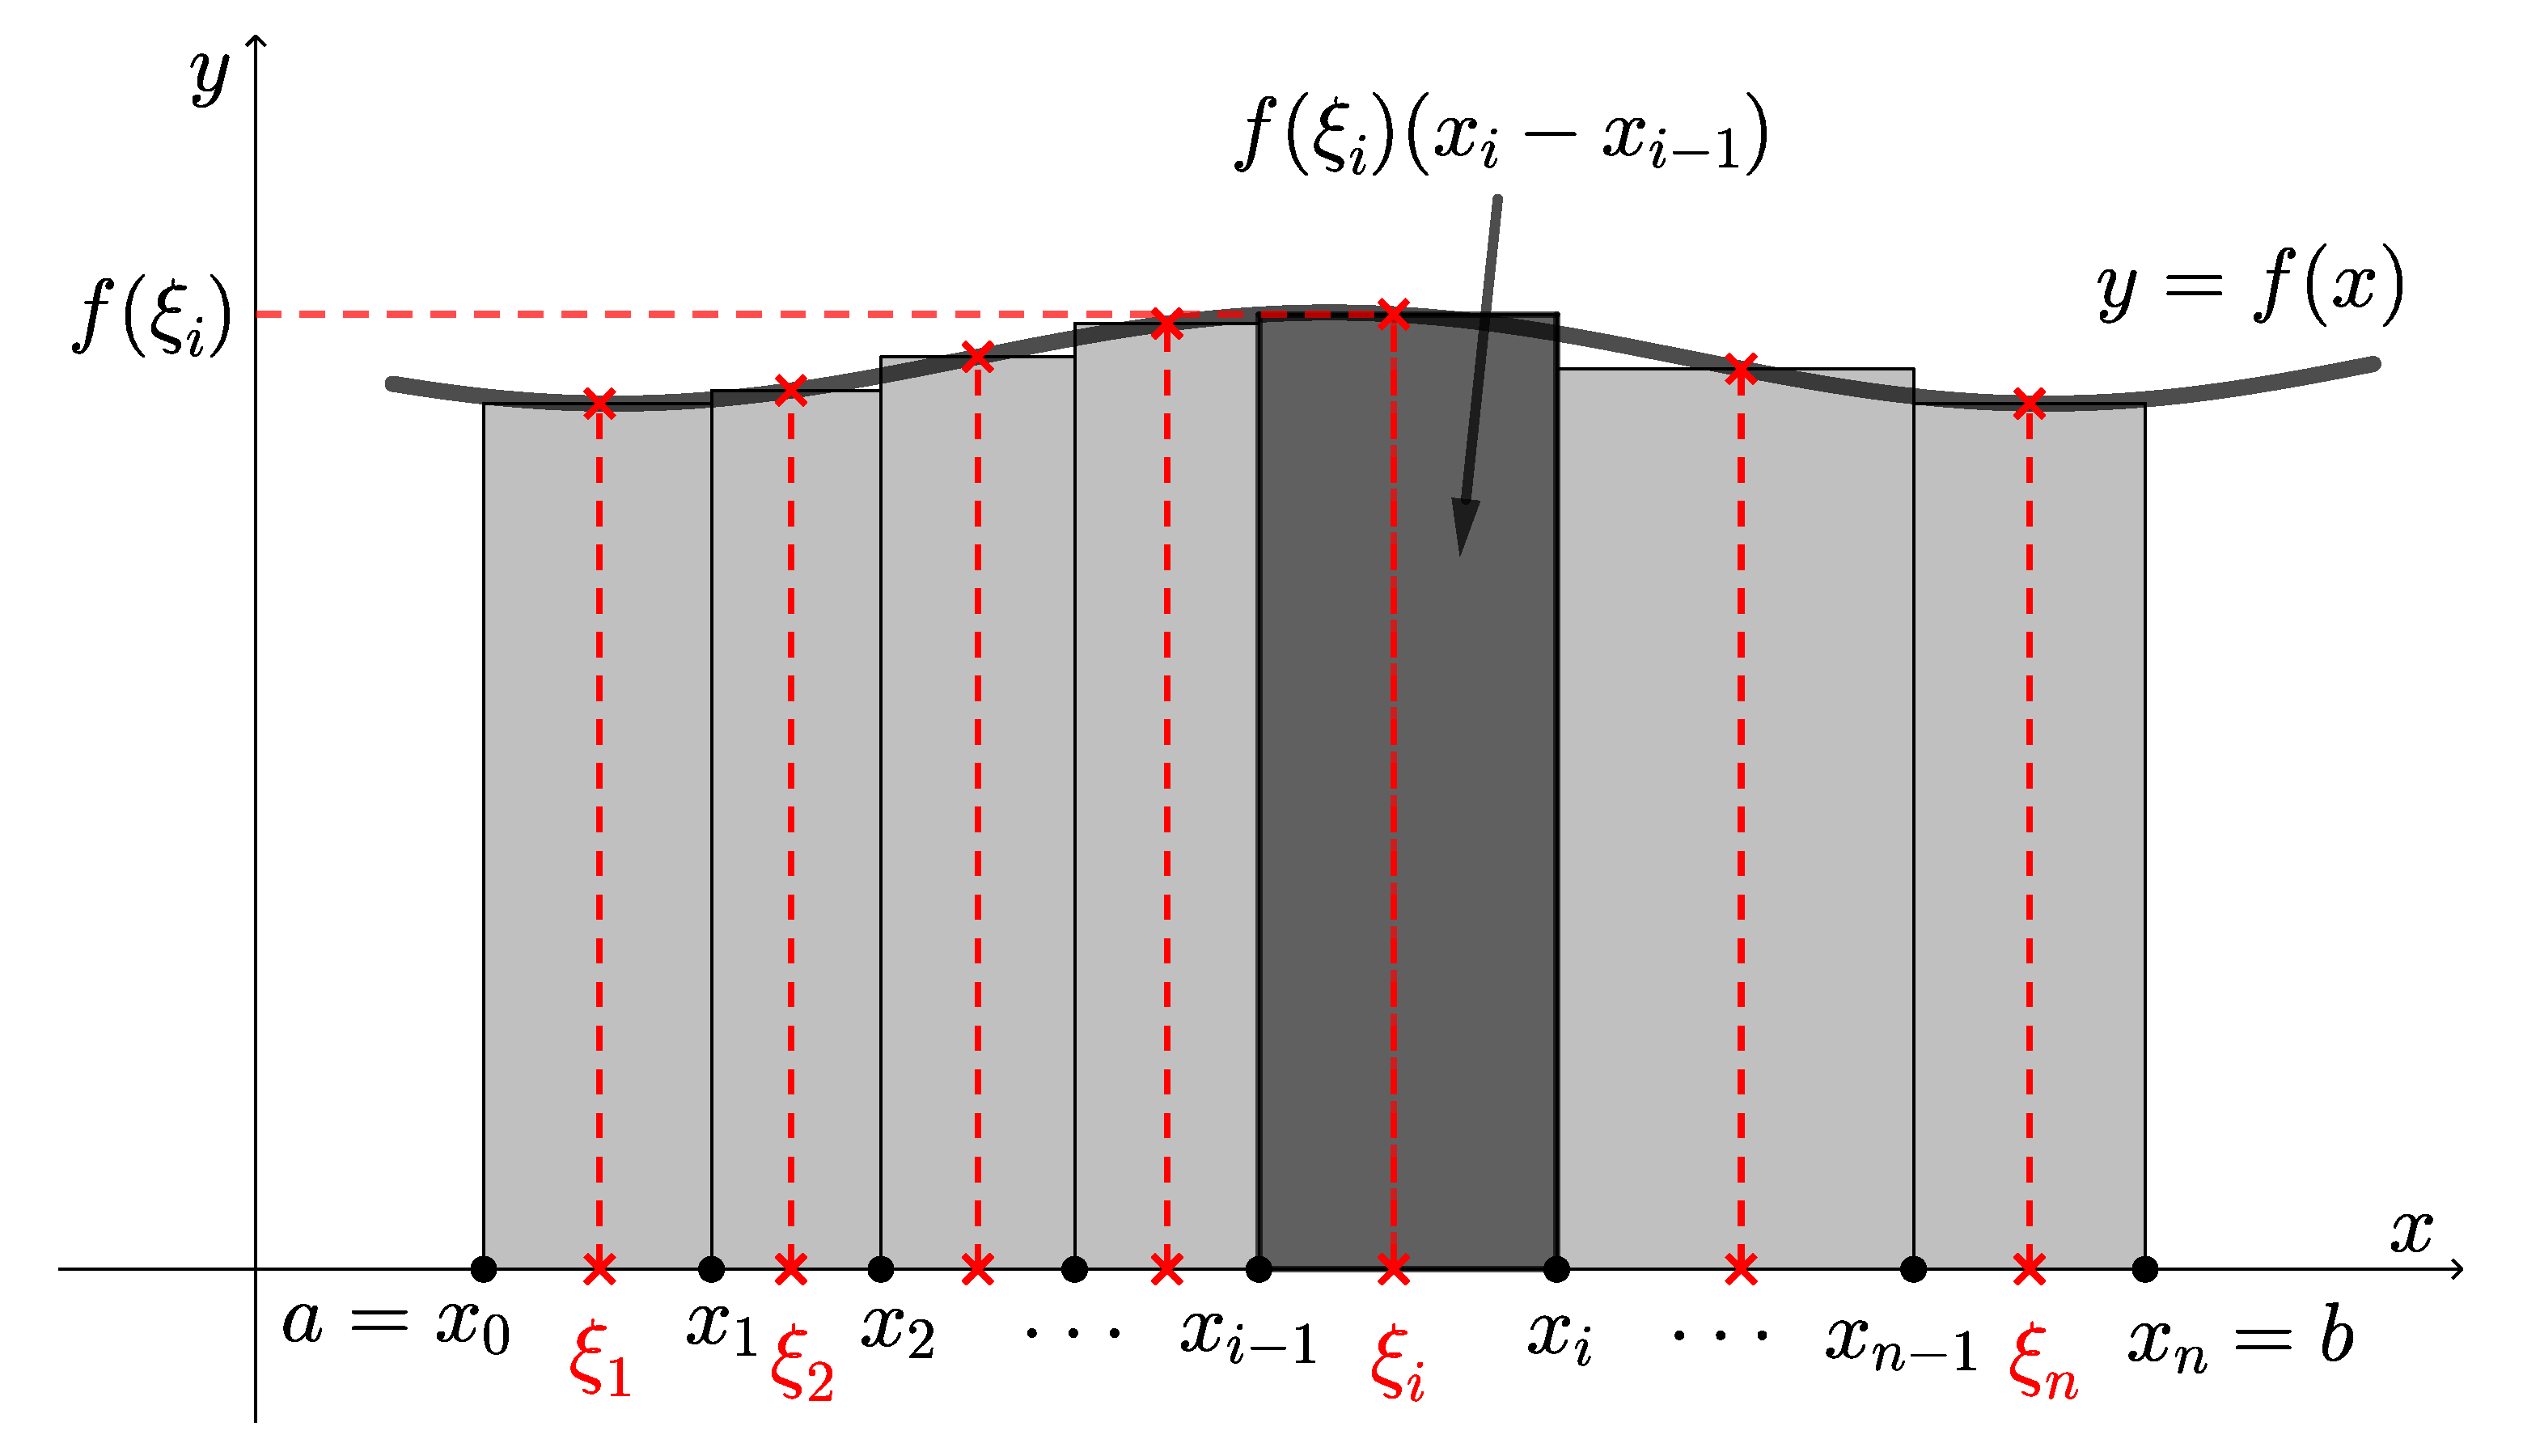
\includegraphics[height=6.5cm]{./pictures/02/RiemannSum.pdf}
  \caption{Riemann 和 $\ds \sum_{i=1}^{n} f(\xi_i)(x_i-x_{i-1})$ は各長
    方形の(符号付き)面積の和に相当する. }\label{fig:RiemannSum1}
\end{figure}

\newpage

簡単な Riemann 和を実際に計算してみよう.

\begin{example}
  $f(x)=x^2$ とする.$\Delta=(x_0,x_1,x_2,x_3,x_4)$ を閉区
  間 $[0,4]$ の $4$ 等分割とし,各小区間 $[ x_{i-1}, x_{i}]$ の中点
  を $\xi_i$ とする.つまり,
  \[
    \Delta=(x_0, x_1, x_2, x_3, x_4) =(0,1,2,3,4), \quad
    \xi_1=\frac{1}{2}, \; \xi_2=\frac{3}{2}, \; \xi_3=\frac{5}{2}, \;
    \xi_4 = \frac{7}{2}
  \]
  とする.これらに関する $f$ の Riemann 和 $R(\Delta, \{\xi_i\}, f)$ を実際に計算してみよう.
  \[
    \begin{aligned}
      R\left( \Delta, \{\xi_i\}, f\right)
      &=f(\xi_1)(x_1-x_0)+f(\xi_2)(x_2-x_1) + f(\xi_3)(x_3-x_2) +
        f(\xi_4)(x_4-x_3)\\[2ex]
      &= f\left(\frac{1}{2}\right) \left( 1-0 \right) + f\left(\frac{3}{2}\right)\left(2-1\right)
        + f\left(\frac{5}{2}\right) \left(3-2\right) + f\left(\frac{7}{2}\right)\left(4-3\right)\\[2ex]
      & = \frac{1}{4} + \frac{9}{4} + \frac{25}{4} + \frac{49}{4} = 21
    \end{aligned}
  \]
\begin{figure}[h]
  \centering
  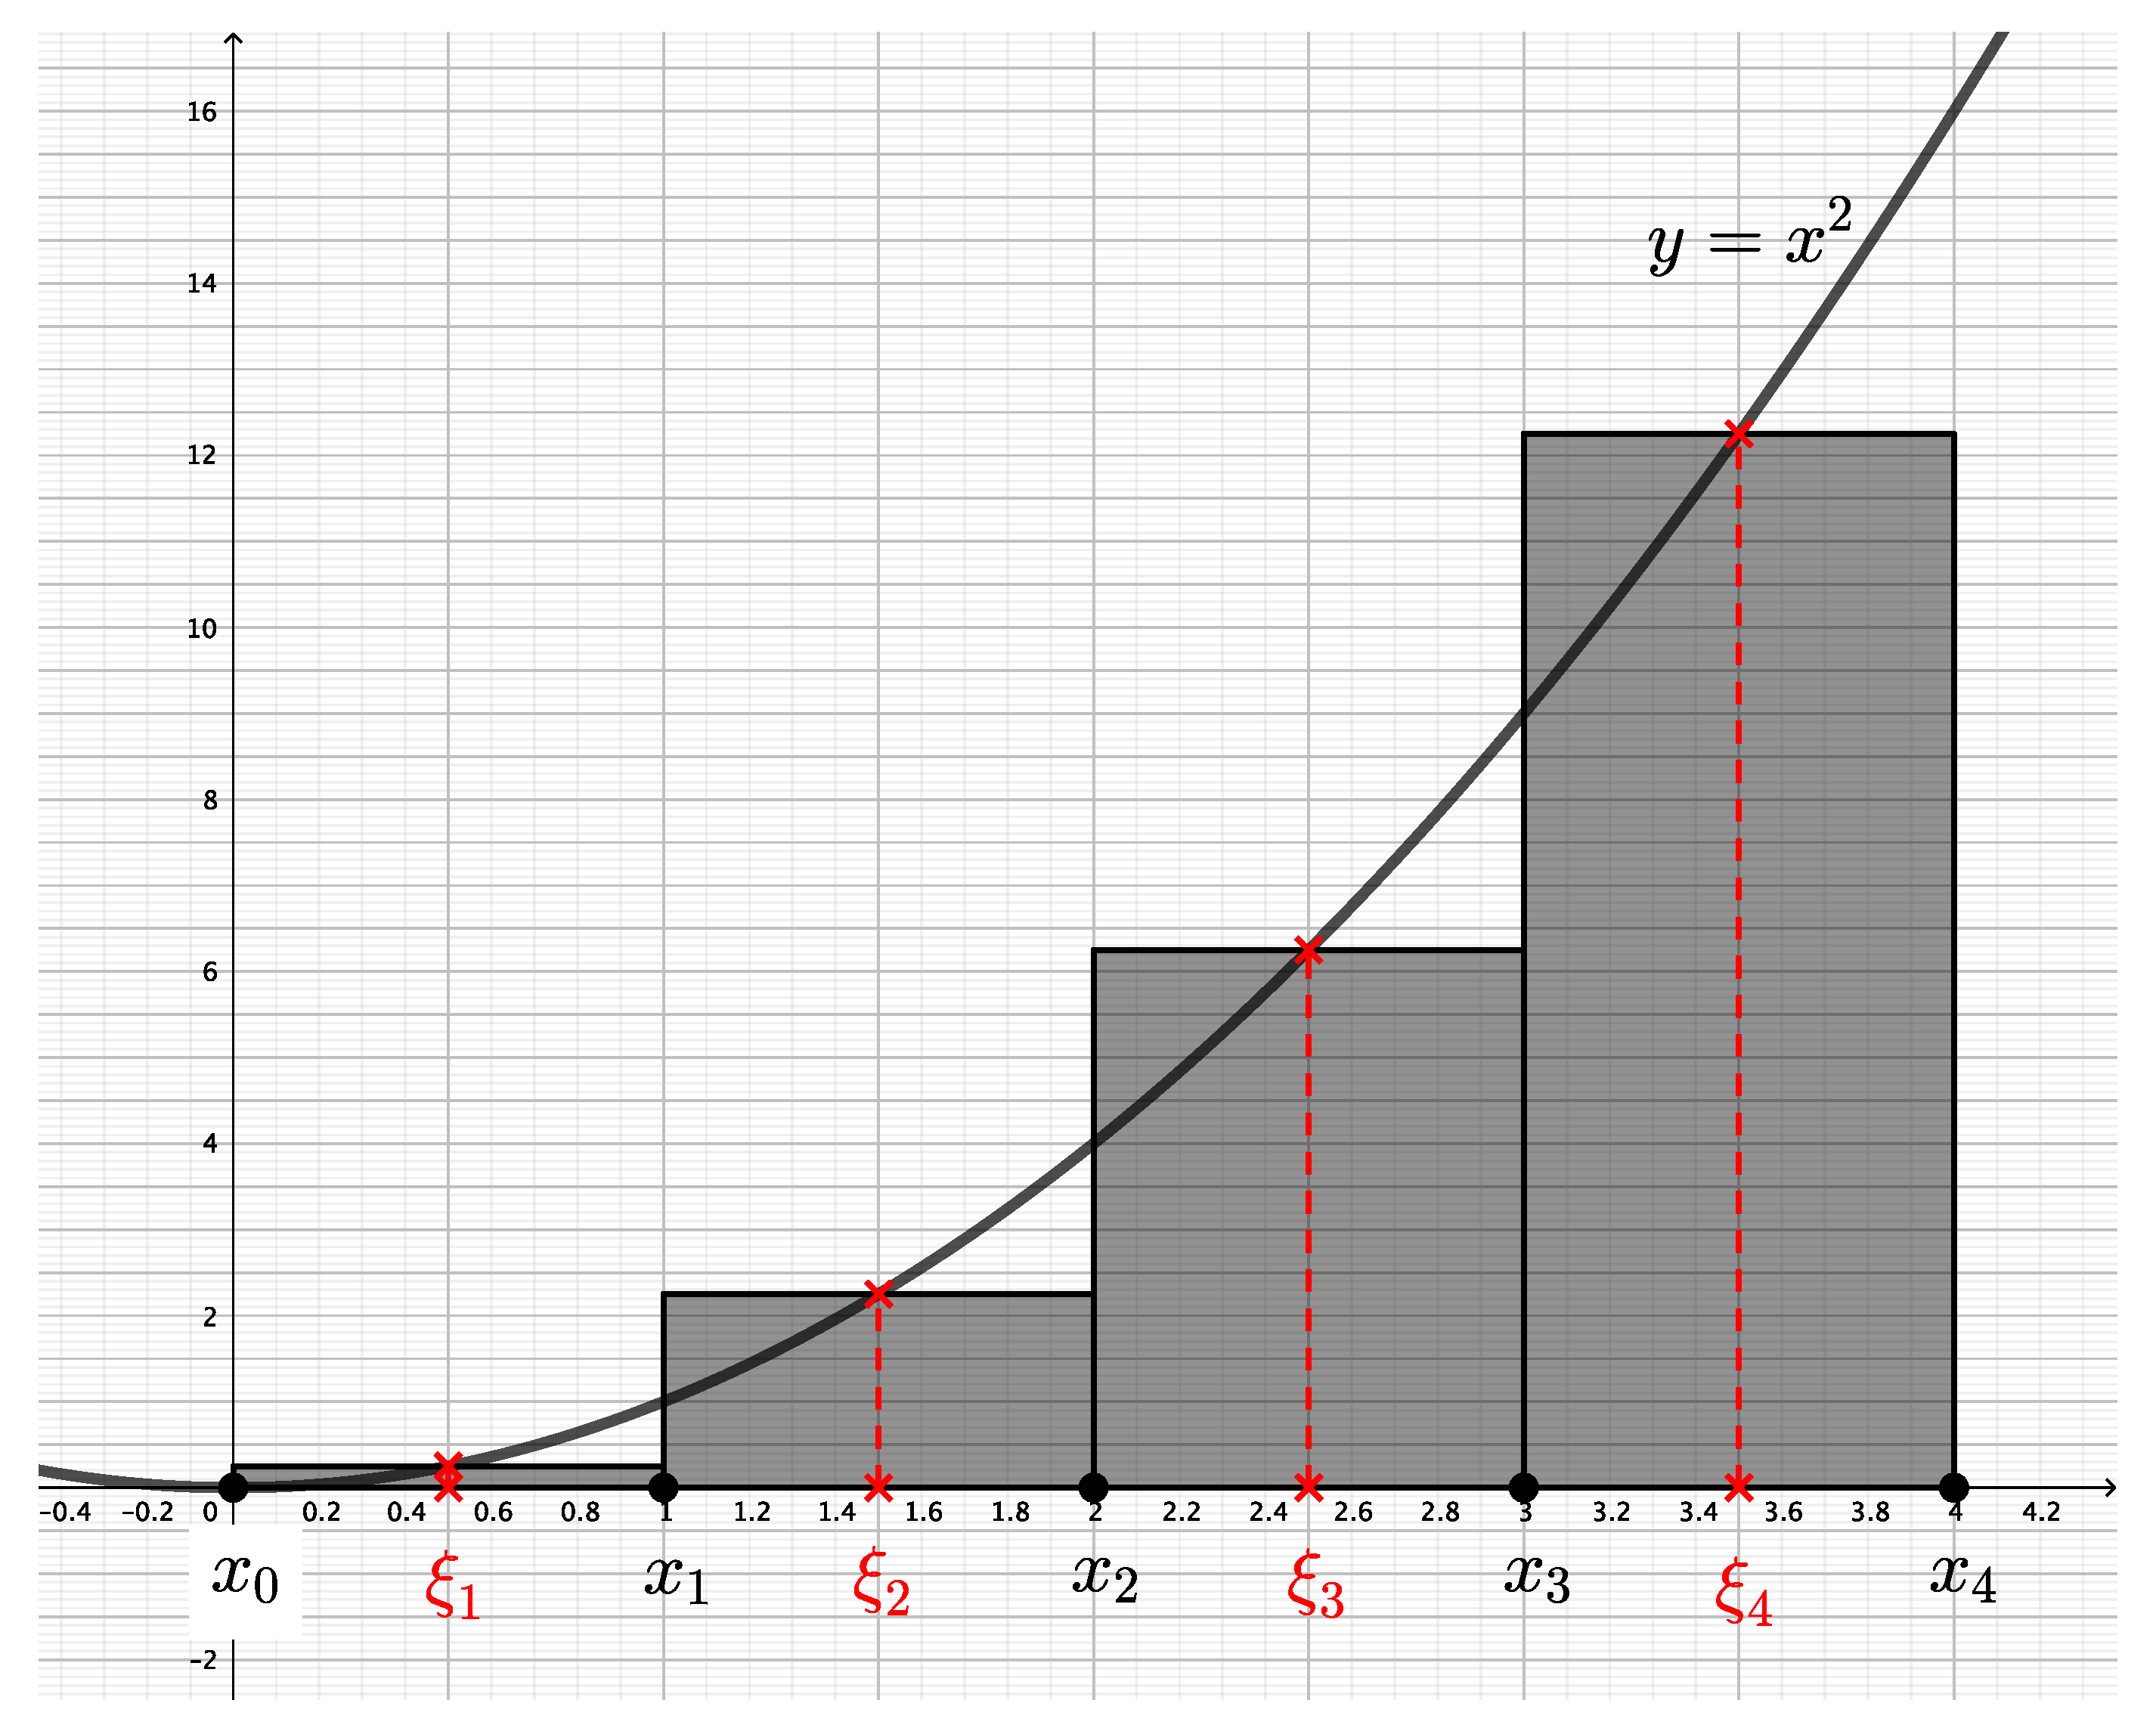
\includegraphics[height=12cm]{./pictures/02/parabola.pdf}
\end{figure}

これは積分 $\ds \int_{0}^{4}x^2 \ dx $ を近似している.実際,後で確認す
るが $\ds \int_{0}^{4} x^2 \ dx = \frac{64}{3} = 21.333\cdots$ である.
\end{example}

\newpage


\subsection{積分の定義}

$f$ を有界閉区間 $[a,b]$ で有界な関数とする.$[a,b]$ の分
割 $\Delta =(x_0, \ldots, x_n)$ に対し,
\[
  |\Delta| := \max_{1 \leq i \leq n}(x_i - x_{i-1})
\]
とする.ここで,$\max$は最大値を意味する.すなわち,$x_1-x_0, x_2-x_1,
\ldots, x_{n}-x_{n-1}$ の中で最も大きな値が $|\Delta|$ であ
る.$|\Delta| \to 0$ のとき,分割の仕方と代表点集合 $\Set{\xi_i}$の選び
方によらず Riemann 和 $R(\Delta, \Set{\xi_i}, f)$ が一定の値に収束する
ならば,$f$ は $[a,b]$ で\textbf{(Riemann) 積分可能},また
は\textbf{(Riemann) 可積分}であるといい,その極限値を
\[
  \int_{a}^{b} f(x) \ dx
\]
で表し,区間 $[a,b]$ における $f$ の\textbf{積分}という.つまり,
\[
  \int_{a}^{b} f(x) \ dx = \lim_{|\Delta| \to 0} \sum_{i=1}^{n} f(\xi_i)(x_i-x_{i-1})
\]
である.ここまでは $a<b$ の場合しか想定していないが,$a \geqq b$ の場合も含めて以下を約束しておく.
\begin{equation}\label{eq:int_promis}
  \int_{a}^{b} f (x) \ dx = - \int_{b}^{a} f(x) \ dx, \qquad \int_{a}^{a} f(x) \ dx =0
\end{equation}


与えられた関数が積分可能であるかどうかを調べるのは容易ではないが,有界
閉区間上の連続関数は積分可能であることが知られている.

\begin{theorem}\label{thm:integrable1}
  有界閉区間 $[a,b]$ 上連続な関数は $[a,b]$ で積分可能である.
\end{theorem}

つまり,積分したい区間で $f$ が連続なら積分できるかどうかは心配する必要
がなく,「どうやって計算するか」のみ考をえればよい.\\

積分の定義から,以下の定理が成り立つ.

\begin{theorem}\label{thm:int_additive}
  $f$ の積分可能な範囲内にある任意の $a,b,c$ に対して以下が成り立つ.
  \[
    \int_{a}^{b} f(x) \ dx + \int_{b}^{c} f(x) \ dx = \int_{a}^{c} f(x) \ dx
  \]
\end{theorem}

\begin{theorem}\label{thm:int_monotomic}
  $f,g$ が区間 $[a,b]$ で積分可能かつ $f(x) \leqq g(x)$ なら $\ds \int_{a}^{b}f(x) \ dx \leqq \int_{a}^{b} g(x) \ dx$ である.
\end{theorem}

一般に,$- |f(x)| \leqq f(x) \leqq | f(x) |$ なので定理\ref{thm:int_monotomic}から以下が成り立つ.
\[
  -\int_{a}^{b} |f(x)| \ dx \leqq \int_{a}^{b} f(x) \ dx \leqq \int_{a}^{b} |f(x)| \ dx
\]
これにより,以下の定理が得られる.

\begin{theorem}\label{thm:int_absolute}
  $f$ が $[a,b]$ で積分可能なら $\ds \left| \int_{a}^{b} f(x) \ dx \right| \leqq \int_{a}^{b} |f(x)| \ dx$ である.
\end{theorem}

\subsection{微分積分学の基本定理}

積分値を定義に基づいて求めるのは大体困難であり,実際には微分積分学の基本定理を使って計算する.

\begin{theorem}[\textbf{微分積分学の基本定理}]\label{thm:fundamental}
  有界閉区間 $[a,b]$ 上の連続関数 $f$ に対して次が成り立つ.
  \begin{enumerate}[(1)]
  \item 関数 $\ds G(x) = \int_{a}^{x} f(t) \
    dt$ は閉区間 $[a,b]$ で定義され,開区間 $(a,b)$ で以下が成り立つ.
    \[
      G'(x)= f(x)
    \]
    つまり,$G$ は $f$ の原始関数である.
    
  \item $f$ の任意の原始関数 $F$ に対して(つまり,$F'=f$ となる任意の $F$ に対して)以下が成り立つ.
    \[
      \int_{a}^{b} f(x) \ dx = F(b) - F(a)
    \]
  \end{enumerate}
\end{theorem}

\begin{remark}
  この定理の(1)は,微分と積分という操作が互いに逆であることを示している.
  これがあるから「微分学」と「積分学」がまとめて「微分積分学」と呼ばれ
  ている.また,(2)は微分の逆操作によって実際に積分の値が計算できること
  を示している.この定理は微分積分学においてもっとも重要
  であり,だからこそ「基本定理」と呼ばれている.\\
\end{remark}

$F(b)-F(a)$ を $\Big[ F(x) \Big]_{a}^{b}$ と書くと便利である.これによって積分の計算は
\[
  \int_{a}^{b}f(x) \ dx = \Big[F(x)\Big]_{a}^{b} = F(a) - F(b) = \cdots 
\]
という形で書かれることが多い.\\

例えば,$\ds \left( \frac{x^3}{3} \right)' = x^3, \; \left( e^x \right)' = e^x$ なので
微分積分学の基本定理(2)から
\[
  \int_{0}^{4} x^2 \ dx = \left[ \frac{x^3}{3} \right]_{0}^{4} = \frac{4^3}{3} - \frac{0^3}{3} = \frac{64}{3}, \qquad
  \int_{0}^{1} e^x \ dx = \left[ e^x \right]_{0}^{1} = e^1 - e^0 = e-1
\]
などと積分の計算が容易に行える.とにかく,$F'=f$ となる $F$ さえ見つかれば積分は容易に計算できる.\\

また,$F'=f$ となる $F$
はどれを選んでもよい.例えば,$\ds \left( \log x \right)' = \left(
  \log (2x) \right)' = \frac{1}{x}$ なので
\[
  \int_{1}^{2} \frac{dx}{x} = \Big[ \log x \Big]_{1}^{2} = \log 2 - \log 1 = \log 2 \quad \Big( F(x) = \log x\Big)
\]
と計算しても
\[
  \int_{1}^{2} \frac{dx}{x} = \Big[\log(2x) \Big]_{1}^{2} = \log 4 - \log 2 = \log\frac{4}{2} = \log 2 \quad
  \Big( F(x) = \log (2x) \Big)
\]
と計算してもよい.ちなみに,$\log (2x) = \log x + \log 2$ なので,$\log x$ と $\log (2x)$ との差は定数 $\log 2$ である.

\subsection{定積分における部分積分と置換積分}

微分積分学の基本定理により,定積分 $\ds \int_{a}^{b} f(x) \ dx$ の計算
の大部分は実質不定積分 $\ds \int f(x) \ dx$ の計算である.そこに部分積分や
置換積分を適用する場合には積分範囲も含めて計算すればよい.\\

定積分で部分積分を適用する場合は,以下のように計算すればよい.
\[
  \int_{a}^{b} f(x)g'(x) \ dx = \Big[ f(x) g(x) \Big]_{a}^{b} - \int_{a}^{b} f'(x) g(x) \ dx
\]

\begin{example}

  \begin{enumerate}[(1)]
    \setlength{\itemsep}{1zh}
    
  \item $\ds \int_{0}^{1} x e^x \ dx = \Big[ x e^x \Big]_{0}^{1} - \int_{0}^{1} e^x \ dx = e -0 - \Big[ e^x \Big]_{0}^{1} =
    e - \left( e-1\right) = 1$

  \item
    $\ds \int_{1}^{2} x \log x \ dx = \left[ \frac{x^2}{2} \log x
    \right]_{1}^{2} - \int_{1}^{2} \frac{x}{2} \ dx = 2 \log 2 - 0 -
    \left[ \frac{x^2}{4} \right]_{1}^{2} = 2 \log 2 - \left( 1 -
      \frac{1}{4}\right) = 2 \log 2 - \frac{3}{4}$
  \end{enumerate}
  
\end{example}

\begin{remark}
  先に不定積分を計算しきってもよい.例えば,上の(1)で
  $\ds \int x e^x \ dx = x e^x - \int e^x \ dx = x e^x - e^x$ と不定積
  分を求めてしまってから以下のように計算してもよい.
  \[
    \int_{0}^{1} x e^x \ dx = \Big[ x e^x - e^x\Big]_{0}^{1} = (e-e) - (0 - 1) = 1
  \]
  これでももちろんよいが,$\ds \int$ が外れたところから代入計算をした方が早く結論に辿りつきやすい.\\
\end{remark}

定積分において,$u=g(x)$ として置換積分を適用する場合には,積分範囲も $u$ の動く範囲に変換する.
\[
  \int_{a}^{b} f\left( g(x) \right) \frac{du}{dx} \ dx = \int_{\alpha}^{\beta} f(u) \ du \quad \left[
    \begin{array}{c|ccc}
      x & a & \to & b \\ \hline
      u & \alpha & \to & \beta
    \end{array}
    \right]
\]

\begin{example}
  $\ds \int_{0}^{\pi/2} \frac{\cos x}{1+\sin x} \ dx$
  
  $u=1+\sin x$ とおくと $\ds \frac{du}{dx} = \cos x$ であり,積分範囲は $
  \begin{array}{c|ccc}
    x & 0 & \to & \pi/2 \\ \hline
    u & 1 & \to & 2
  \end{array}$ と変換される.
  \[
    \int_{0}^{\pi/2} \frac{\cos x}{1+\sin x} \ dx = \int_{0}^{\pi/2} \frac{1}{u}~ \frac{du}{dx} \ dx
    = \int_{1}^{2} \frac{du}{u} = \Big[ \log u \Big]_{1}^{2} = \log 2
  \]
\end{example}

\begin{remark}
  上の例で,先に不定積分を
  $\ds \int \frac{\cos x}{1+\sin x} \ dx = \int \frac{du}{u} = \log |u| = \log |1+\sin x|$ と計算しきってから
  \[
    \int_{0}^{\pi/2} \frac{\cos x}{1+\sin x} \ dx = \Big[ \log |1+\sin x| \Big]_{0}^{\pi/2}
    = \log 2 - \log 1 = \log 2
  \]
  と計算してももちろんよいが,積分範囲も変換しながら計算すれば,不定積分を計算しきる必要がなくなる.
\end{remark}


具体的な積分計算は以下のリンク先の「積分基本問題集 壱」(1) $\sim$ (26) で練習してください.
\begin{center}
  \url{https://github.com/kazutsumi/Integral1/blob/main/integral1.pdf}

  (表紙にQRコードがあります)
\end{center}



\subsection{微分積分学の基本定理の証明}

微分積分学の基本定理(定理\ref{thm:fundamental})は微分積分学において最
も重要な定理なのでその証明を書いておく.興味がなければ読み飛ばしてもよ
い.なお,基本的に教科書と同じ証明である.

\begin{fundamental}
  有界閉区間 $[a,b]$ 上の連続関数 $f$ に対して次が成り立つ.
  \begin{enumerate}[(1)]
  \item 関数 $\ds G(x) = \int_{a}^{x} f(t)\ dt$ は閉区間 $[a,b]$ で定義され,開区間 $(a,b)$ で以下が成り立つ.
    \[
      G'(x) = f(x)
    \]
    
  \item $f$ の任意の原始関数 $F$ に対して以下が成り立つ.
    \[
      \int_{a}^{b} f(x) \ dx = F(b) - F(a)
    \]
  \end{enumerate}
\end{fundamental}

\vspace{1zh}

まず,(1)を認めてしまえば以下の補題\ref{lem:uptoC}から(2)は容易に示せる.

\begin{lemma}\label{lem:uptoC}
  $F,G$ を有界閉区間 $[a,b]$ 上の連続関数 $f$ の原始関数とする.このと
  き,$F(x) = G(x) +C$ となる定数 $C$ が存在する.
\end{lemma}

\begin{proof}
  $H(x) = F(x) - G(x)$ とする.$H'(x) = F'(x) - G'(x) = f(x) - f(x) =
  0$ なので,$H$ は $[a,b]$ 上の定数関数である.実際,平均値の定理から
  任意の $x_1 ,x_2 \in [a,b] \; ( x_1 < x_2)$ に対して
  \[
    \frac{H(x_2) - H(x_1)}{x_2-x_1} = H'(c) , \quad x_1 < c < x_2
  \]
  となる実数 $c$ が存在するが,$H'(c)=0$ なので $H(x_1) =
  H(x_2)$ より $H$ は定数関数である.よって,$H(x) = F(x) - G(x) = C$
  となる定数 $C$ が存在する.これより,$F(x) = G(x) +C$ である.
\end{proof}

\vspace{1zh}

\begin{proof}[微分積分学の基本定理(2)の証明]
  (1)から $G(x)$ は $f$ の原始関数なので,補
  題\ref{lem:uptoC}から $F(x) = G(x) +C$ を満たす定数 $C$ が存在する.
  また,$\ds \int_{a}^{a} f(t) \ dt =0$ と約束しているので
  \[
    F(b) - F(a) = \Big(G(b) +C \Big) - \Big(G(a) +C\Big) = G(b) - G(a)
    = \int_{a}^{b} f(t) \ dt - \int_{a}^{a} f(t) \ dt = \int_{a}^{b} f(x) \ dx
  \]
  である.なお,変数に使う文字によって積分値は変わらないので
  $\ds \int_{a}^{b} f(t) \ dt = \int_{a}^{b} f(x) \ dx$ である.
\end{proof}

\newpage

次に,定理\ref{thm:int_additive}と以下の補題\ref{lem:int_average}から微分積分学の基本定理(1)を証明する.

\begin{lemma}[\textbf{積分の平均値の定理}]\label{lem:int_average}
  有界閉区間 $[a,b]$ 上の連続関数 $f$ に対し,以下を満たす実数 $c$ が存在する.
  \[
    \int_{a}^{b}f(x) \ dx = f(c)(b-a), \quad a < c < b
  \]
\end{lemma}

\begin{proof}
  $f$ が定数関数なら明らかなので,$f$ は定数関数でないとする.$f$ は閉
  区間 $[a,b]$ で連続なので最小値 $m$ と最大値 $M$ が存在する.それらを
  実現する値をそれぞれ $x_{\min}, x_{\max} \in [a,b]$ とする.つま
  り,$f(x_{\min})=m, \; f(x_{\max})=M$ である.$f$ は定数関数でないの
  で $x_{\min} \neq x_{\max}$ である.定理\ref{thm:int_monotomic}より
  \[
    m(b-a) = \int_{a}^{b} m \ dx \leqq \int_{a}^{b} f(x) \ dx \leqq \int_{a}^{b} M \ dx = M (b-a)
  \]
  が成り立つ.これより
  \[
    m \leqq \frac{1}{b-a} \int_{a}^{b} f(x) \ dx \leqq M
  \]
  である.よって,中間値の定理から
  \[
    \frac{1}{b-a} \int_{a}^{b} f(x) \ dx = f(c), \quad x_{\min} < c < x_{\max} \text{ または } x_{\max} < c < x_{\min}
  \]
  を満たす実数 $c$ が存在する.従って,
  \[
    \int_{a}^{b} f(x) \ dx = f(c) (b-a)
  \]
  である.ここで,$x_{\min}, x_{\max} \in [a,b]$ なので $a < c < b$ である.
\end{proof}

\vspace{1zh}

\begin{proof}[微分積分学の定理(1)の証明]
  $x \in (a,b)$ とする.定理\ref{thm:int_additive}と約束 (\ref{eq:int_promis}) から
  \[
    \begin{aligned}
      \frac{G(x+h) - G(x)}{h}
      &= \frac{1}{h}\left(\int_{a}^{x+h}f(t) \ dt - \int_{a}^{x} f(t) \ dt\right)
        \underset{(\ref{eq:int_promis})}{=}\frac{1}{h} \left( \int_{a}^{x+h} f(t) \ dt + \int_{x}^{a} f(t) \ dt \right)\\
      &\underset{\text{定理\ref{thm:int_additive}}}{=} \frac{1}{h} \int_{x}^{x+h} f(t) \ dt
    \end{aligned}
  \]
  である.さらに,補題\ref{lem:int_average}から
  \[
    \int_{x}^{x+h} f(t) \ dt = f(c)h
  \]
  を満たす実数 $c$ が $x$ と $x+h$ の間に存在するので
  \[
    \frac{G(x+h) - G(x)}{h} = f(c)
  \]
  である.$h \to 0$ のとき $c \to x$ であり,$f$ は連続なので
  \[
    G'(x) = \lim_{h \to 0} \frac{G(x+h)-G(x)}{h} = \lim_{c \to x} f(c) = f(x)
  \]
  である.つまり,$G$ は開区間 $(a,b)$ で微分可能で $G'(x) = f(x)$ である.
\end{proof}
\newpage

\subsection{(おまけ)Riemann 和の極限としての積分}\label{sec:Rsum_computation}
有界閉区間上の連続関数の積分の値を Riemann 和の極限としていくつか計算する.

\begin{example}
$\ds \int_{0}^{4} x^2 \ dx$ 

  \vspace{1zh}

  $\Delta_n=(x_0, \ldots, x_n)$ を閉区間 $[0,4]$ の $n$ 等分割,各小区間 $[x_{i-1}, x_i]$
  の中点を代表点 $\xi_i$ とする.つまり,
  \[
    x_i = \frac{4i}{n} \; (i=0,1, \ldots, n) , \qquad \xi_i =
    \frac{x_{i-1} + x_{i}}{2} = \frac{2(2i-1)}{n} \; (i=1,2, \ldots, n)
  \]
  とする.これらに関する $f(x) =
  x^2$ の Riemann 和を $S_n$ とする.これは図\ref{fig:Rsum_quadratic}の灰色部分の面
  積に等しい.
  \begin{figure}[h]
    \centering
    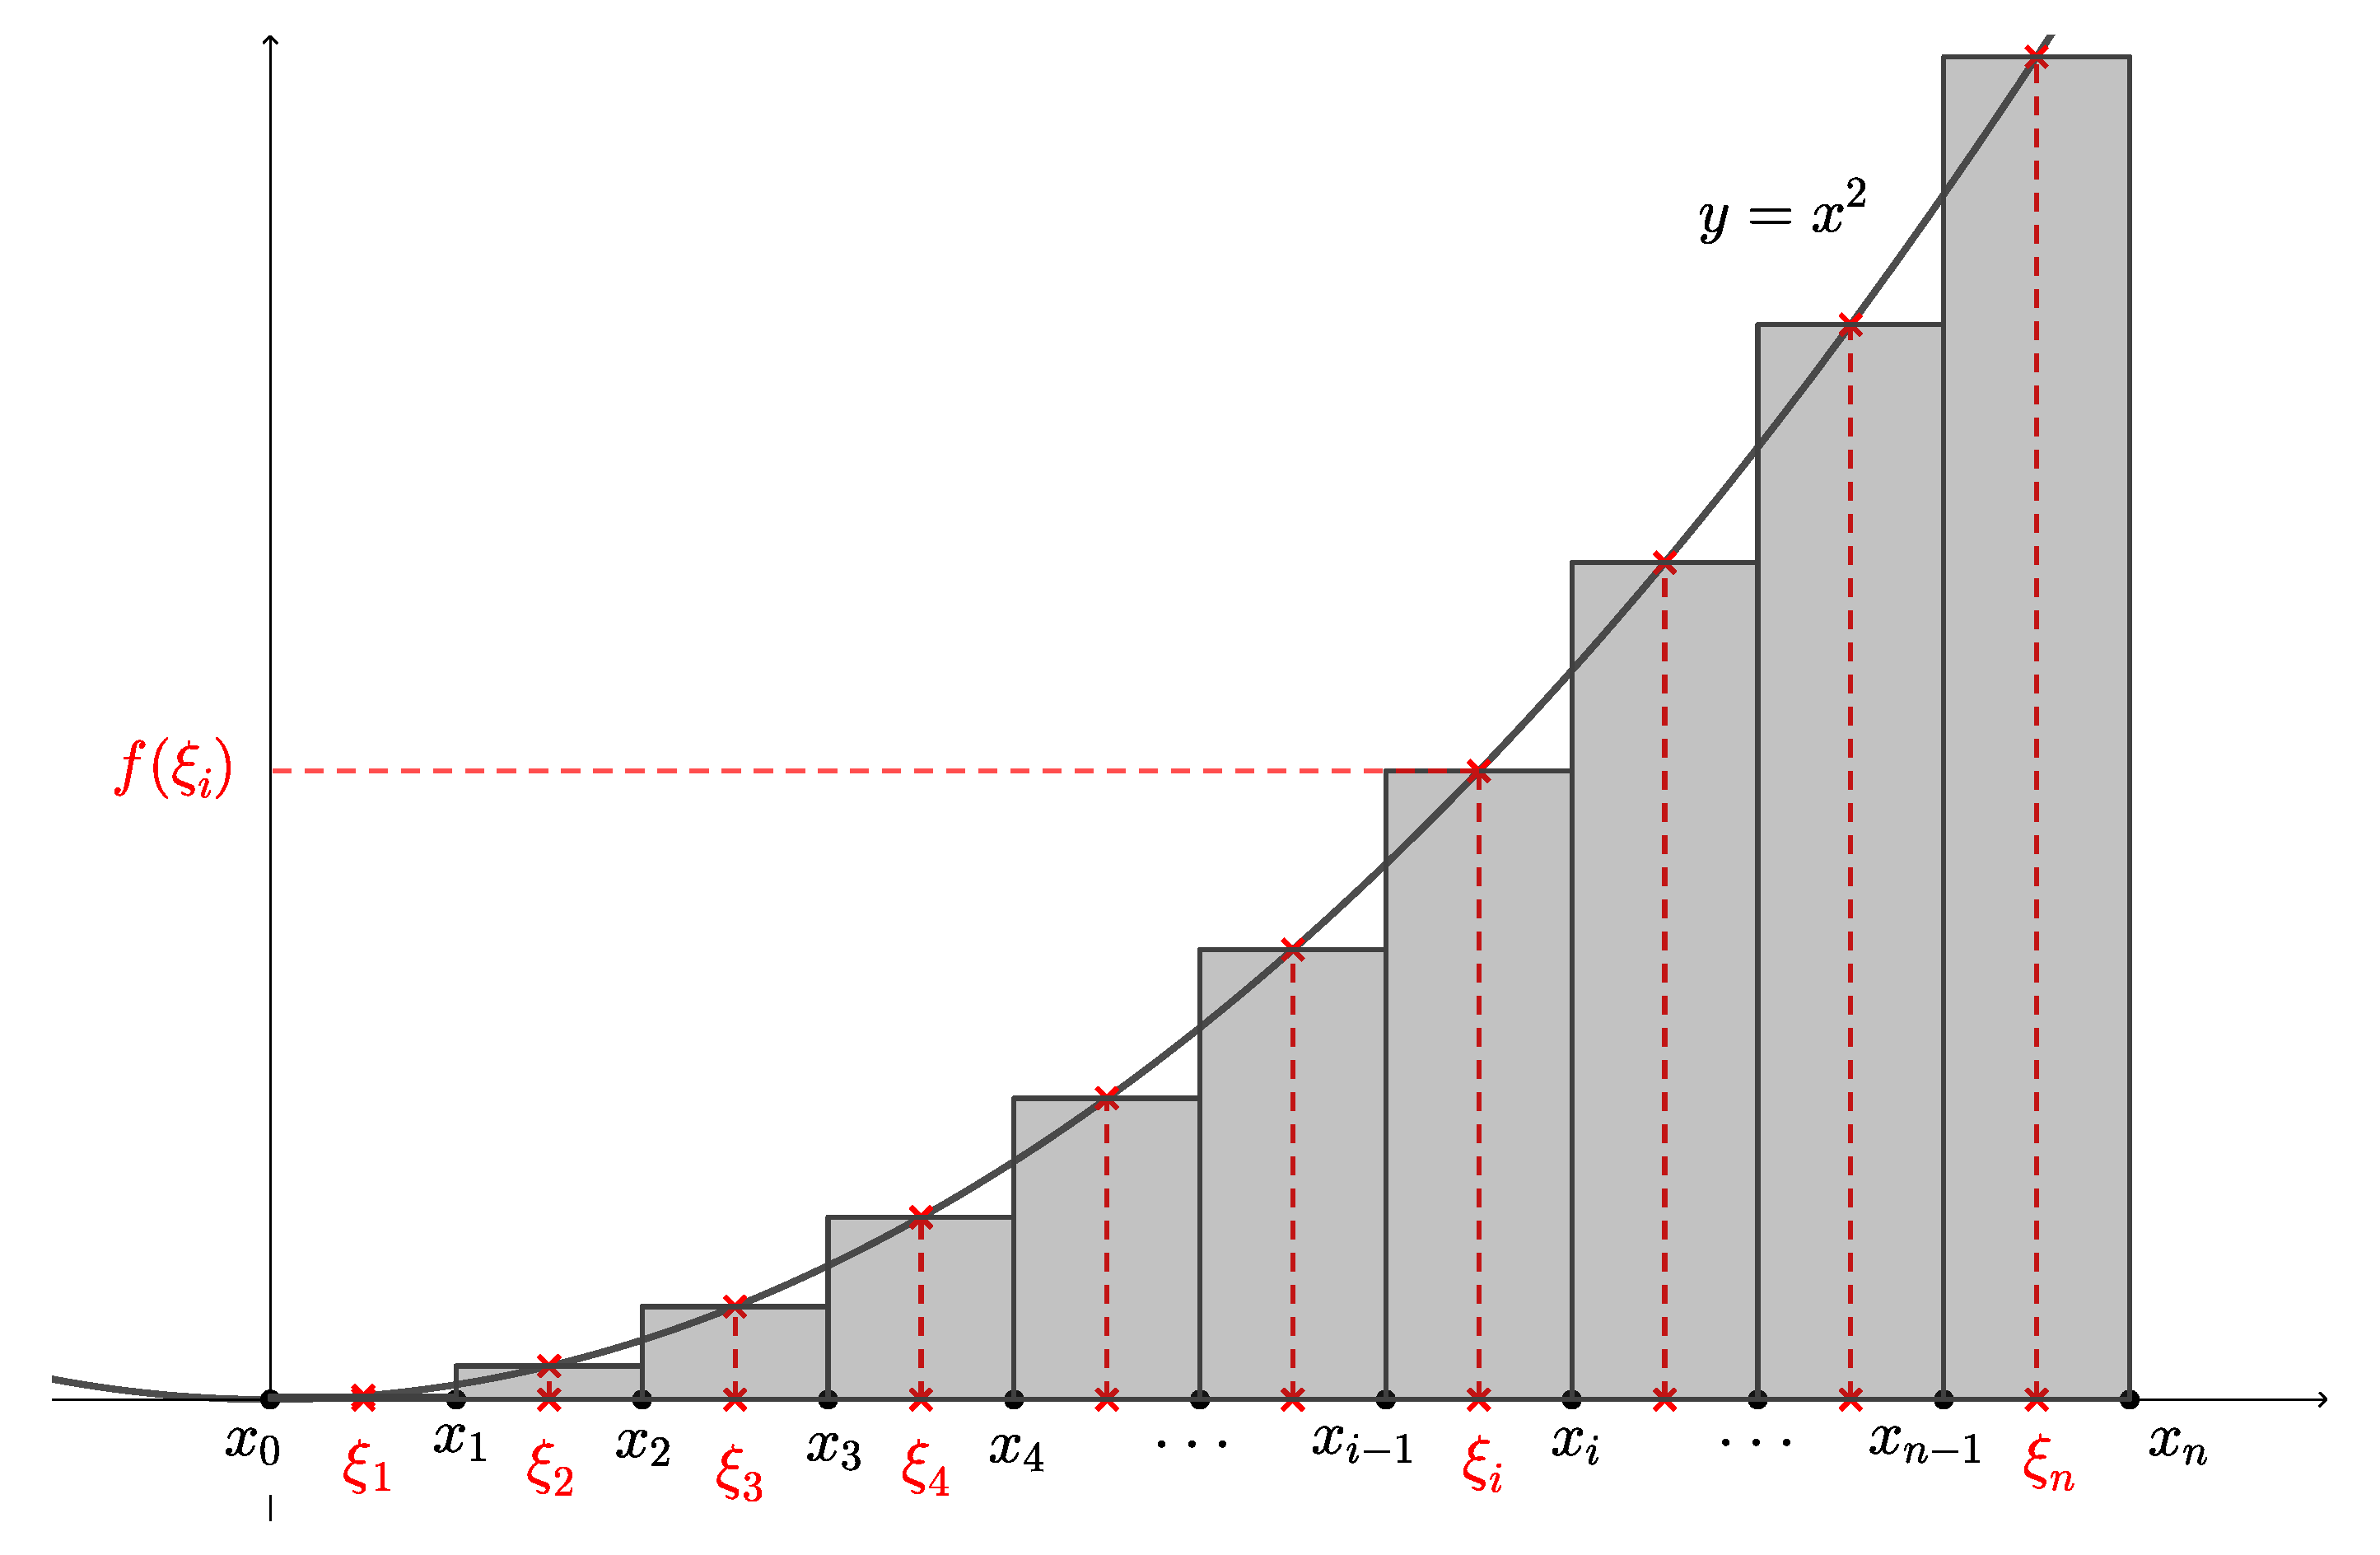
\includegraphics[height=8cm]{./pictures/02/quadratic.pdf}
    \caption{}\label{fig:Rsum_quadratic}
  \end{figure}
  $n \to \infty$ のとき,$|\Delta_n| \to 0$ だから定理\ref{thm:integrable1}より $S_n$ は
  収束し,その極限値が求める積分値である.

  Riemann 和 $\ds S_n $ を具体的に計算する.$\Delta_n$ は区間 $[0,4]$ の $n$ 等
  分割なので,各 $i$ で $\ds x_{i} - x_{i-1} = \frac{4}{n}$ である.
  \[
    \begin{aligned}
      S_n &= \sum_{i=1}^{n} f(\xi_i)(x_i - x_{i-1})
            = \sum_{i=1}^{n} \left( \frac{2(2i-1)}{n}\right)^2 \cdot \frac{4}{n}
            =\frac{16}{n^3}\sum_{i=1}^{n} (2i-1)^2
            = \frac{16}{n^3} \sum_{i=1}^{n} \left(4i^2-4i+1\right)\\[2ex]
          &  = \frac{16}{n^3} \left( 4 \sum_{i=1}^{n} i^2 - 4 \sum_{i=1}^{n} i + \sum_{i=1}^{n} 1\right)
            = \frac{16}{n^3} \left( 4 \cdot \frac{n(n+1)(2n+1)}{6} - 4 \cdot \frac{n(n+1)}{2} + n\right)\\[2ex]
          &= 16 \left( \frac{2}{3} \left( 1 + \frac{1}{n}\right)\left(2+\frac{1}{n}\right)
            - \frac{2}{n} \left(1+\frac{1}{n}\right) + \frac{1}{n^2}\right) \to \frac{64}{3} \; (n \to \infty)
    \end{aligned}
  \]
  これより,$\ds \int_{0}^{4}x^2 \ dx = \lim_{n \to \infty} S_n = \frac{64}{3}$ である.
\end{example}

\newpage

\begin{example}
  $\ds \int_{0}^{1} e^x \ dx$ 

  \vspace{1zh}
  
  $\Delta_n=(x_0,\ldots, x_n)$ を閉区間 $[0,1]$ の $n$ 等分割,各小区間 $[x_{i-1},x_i]$ の
  右端 $x_i$ を代表点 $\xi_i$ とする.つまり,
  \[
    x_i = \xi_i = \frac{i}{n}
  \]
  とする.これらにに関する $f(x) = e^x$ の Riemann和を $S_n$ とする.こ
  れは図\ref{fig:Rsum_exp}の灰色部分の面積に等しい.$n \to \infty$ のと
  き,$|\Delta_n| \to 0$ だから定理\ref{thm:integrable1}より $S_n$ は収束し,その極限値が求める積分
  値である.
  \begin{figure}[h]
    \centering
    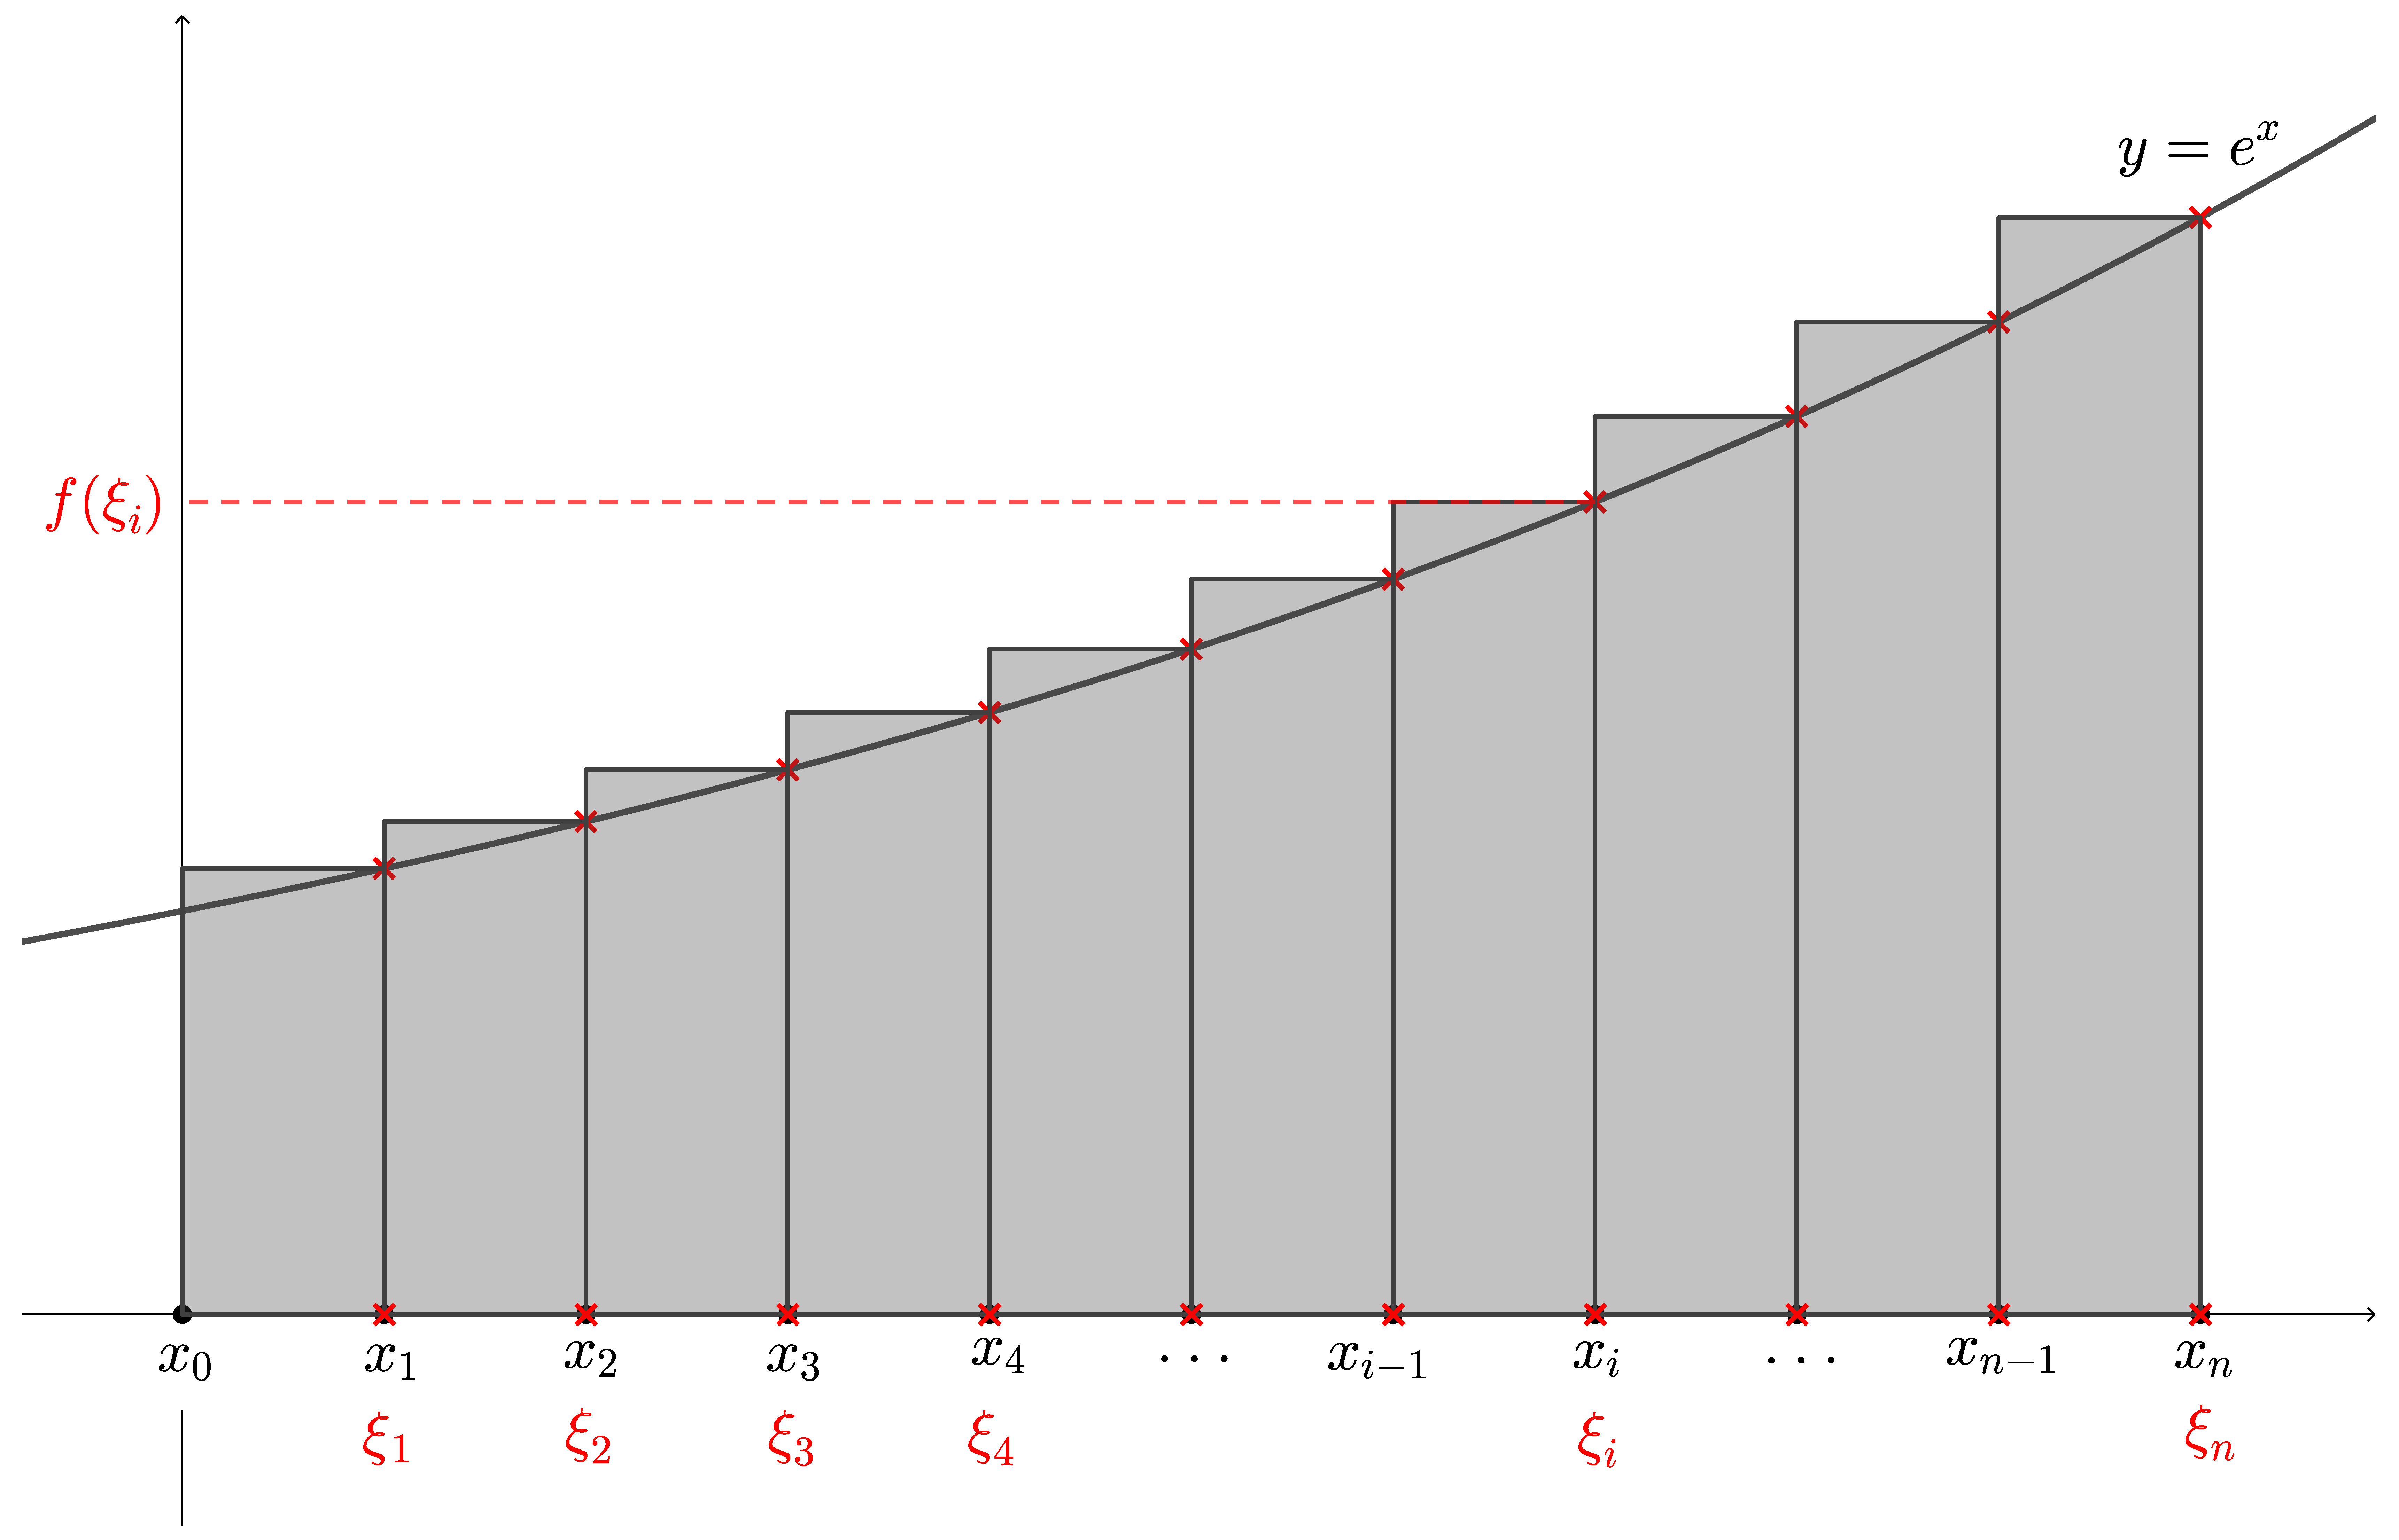
\includegraphics[height=8cm]{./pictures/02/exp.pdf}
    \caption{}\label{fig:Rsum_exp}
  \end{figure}
\end{example}

Riemann 和 $S_n$ を具体的に計算する.$\Delta_n$ は区間 $[0,1]$ の $n$ 等分割な
ので,各 $i$ で $\ds x_i-x_{i-1} = \frac{1}{n}$ である.
\[
  \begin{aligned}
    S_n &= \sum_{i=1}^{n} f(\xi_i) (x_i-x_{i-1}) = \sum_{i=1}^{n} e^{\frac{i}{n}} \cdot \frac{1}{n}\\[2ex]
        & = \frac{1}{n} \left( e^{\frac{1}{n}}
          + \left(e^{\frac{1}{n}}\right)^2 + \left( e^{\frac{1}{n}}\right)^3 +\cdots
          + \left( e^{\frac{1}{n}}\right)^n\right) \quad \left( \text{ 公比 $e^{\frac{1}{n}}$ の等比級数}\right)\\[2ex]
        & = \frac{1}{n} \cdot \frac{e^{\frac{1}{n}} \left( 1 - \left( e^{\frac{1}{n}}\right)^n\right)}{1-e^{\frac{1}{n}}}
          = \frac{e^{\frac{1}{n}}}{n} \cdot \frac{e-1}{e^{\frac{1}{n}}-1}
  \end{aligned}
\]
ここで,$\ds t=e^{\frac{1}{n}}-1$ とおく.これにより $\ds \frac{1}{n} = \log(1+t)$ なので,
\[
  S_n = \frac{\log(1+t)}{t} \cdot (e-1)(t+1) = (e-1) (t+1) \log(1+t)^{\frac{1}{t}}
\]
と変形できる.$n \to \infty$ のとき $t \to +0$ なので,$\ds \lim_{t \to +0} \log (1+t)^{\frac{1}{t}}=1$ と合わせて以下を得る.
\[
  \int_{0}^{1} e^x \ dx = \lim_{n \to \infty} S_n = (e-1) \lim_{t\to +0} (t+1) \log (1+t)^{\frac{1}{t}} = e-1
\]


定数関数 $f(x) = C$ は連続関数だが,定理\ref{thm:integrable1}に頼ることなく直接積分を計算できる.
\begin{example}
  $\ds \int_{a}^{b} C \ dx$\\

  $\Delta = (x_0, \ldots, x_n)$ を閉区間 $[a,b]$ の任意の分割とし,各小
  区間の $[x_{i-1}, x_{i}]$ の代表点 $\xi_i$ を任意に選ぶ.これらに関す
  る $f(x) = C$ の Riemann 和は
  \[
    \begin{aligned}
      R(\Delta, \{\xi_i\}, f) &= \sum_{i=1}^{n} f(\xi_i) (x_i - x_{i-1}) = \sum_{i=1}^{n} C (x_{i}-x_{i-1})\\[2ex]
                              & = C \Big( (x_1-x_0) + (x_2-x_1) + \cdots + (x_n-x_{n-1}) \Big)
                                = C(x_n-x_0) = C(b-a)
    \end{aligned}
  \]
  である.よって,分割の仕方と代表点の選び方によらず Riemann 和は一定な
  ので,特に $|\Delta|\to 0$ における極限値もその一定の値に等しい.よっ
  て,$\ds \int_{a}^{b} C \ dx = \lim_{|\Delta| \to 0} R(\Delta, \{\xi_i\}, f) = C(b-a)$ である.
\end{example}

\newpage

\section{分数関数の積分}

$\ds \frac{\text{多項式}}{\text{多項式}}$ という形をした関数
は\textbf{分数関数}とか\textbf{有理関数}と呼ばれる.その積分の計算方法をまとめる.
% \[
%   \int \frac{dx}{(x-\alpha)^n}, \qquad \int \frac{Bx+C}{(x^2+bx+c)^n}\ dx
%   \qquad (n \text{ は自然数 })
% \]

\subsection{多項式の割り算}\label{subsec:division}

\begin{wrapfigure}{r}[0pt]{0.5\textwidth}
  \centering
  \includegraphics[width=8cm]{./pictures/03/remainder.pdf}
\end{wrapfigure}
例えば,次のような分数関数 $f(x)$ を積分したい.
\[
  f(x) = \frac{x^5+3x^3-2x+1}{x^2+3x+2}
\]
この分子と分母の多項式としての次数を比べると
\[
  \text{ 分子の次数 }  \geqq \text{ 分母の次数} 
\]
である.このような場合は,まず右のように分子を分母で割った商と余
りを計算しておく.この計算により $f(x)$ の分子が
\[
  x^5+3x^3-2x+1 = (x^3-3x^2+10x-24)(x^2+3x+2) + 50x+49
\]
と書けるので
\[
  f(x) = \frac{ (x^3-3x^2+10x-24)(x^2+3x+2) + 50x+49}{x^2+3x+2} = x^3-3x^2+10x-24 + \frac{50x+49}{x^2+3x+2}
\]
と変形できる.よって,$f(x)$ の積分は
\[
  \int f(x) \ dx = \frac{1}{4}x^4 - \frac{2}{3}x^3-5x^2-24x + \int
  \frac{50x+49}{x^2+3x+2} \ dx
\]
となり,もともとの $\ds \frac{\text{ $5$ 次式}}{\text{ $2$ 次式}}$ の積
分が $\ds \frac{\text{$1$ 次式}}{\text{$2$ 次式}}$ の積分に帰着されている.より一般に,分数関数が
\[
  f(x) = \frac{g(x)}{h(x)}
\]
と,$2$ 個の多項式 $g(x)$ と $h(x)$ の比で書けるとき,多項式の割り算を実行して
\[
  g(x) = q(x) h(x) + r(x), \quad \deg r(x) < \deg h(x)
\]
を満たす多項式 $q(x)$ と $r(x)$ を計算することができる.$q(x)$ が商
で,$r(x)$ が余りである.ただし,初めから $\deg g(x) < \deg h(x)$ であ
れば,$q(x)=0, \; r(x) = h(x)$ である.これらによって
\[
  f(x) = \frac{q(x)h(x)+r(x)}{h(x)} = q(x) + \frac{r(x)}{h(x)}
\]
と,$f(x)$ を「多項式」と「分子の次数 $<$ 分母の次数となる分数関数」の和に分けることができる.つまり,
\[
  \text{ 分子の次数 } < \text{ 分母の次数}
\]
となる分数関数の積分が計算できれば,原理的にはどんな分数関数の積分も計算できる.

\subsection{部分分数分解}\label{subsec:partfrac}

分数関数 $\ds f(x) = \frac{x^5+3x^2-2x+1}{x^2+3x+2}$ の積分を完成させよう.先ほど見たように
\[
  \int f(x) \ dx = \frac{1}{4}x^4-\frac{2}{3}x^3-5x^2-24x + \int \frac{50x+49}{x^2+3x+2} \ dx
\]
なので,最後に残った積分
\[
  \int \frac{50x+49}{x^2+3x+2}\ dx
\]
を計算してしまえばよい.まず,分母が
\[
  \frac{50x+49}{x^2+3x+2} = \frac{50x+49}{(x+1)(x+2)}
\]
と因数分解できる.これをさらに
\[
  \frac{50x+49}{(x+1)(x+2)} = \frac{A}{x+1} + \frac{B}{x+2}
\]
という簡素な分数関数の和に分けることができる.特に,左辺が
\[
  \text{ 分子の次数 } < \text{ 分母の次数}
\]
なので,右辺に並ぶ分数関数も全てそうなる.従って,$A, B$ は共に $0$ 次,つまり定数である.実際,
上式の右辺を通分すれば
\[
  \frac{A}{x+1} + \frac{B}{x+2} = \frac{A(x+2)+B(x+1)}{(x+1)(x+2)} = \frac{(A+B)x + (2A+B)}{(x+1)(x+2)}
\]
となるので,分子の係数を比較して以下の連立1次方程式を解けばよい.
\[
  \begin{cases}
    A+B=50\\
    2A+B=49
  \end{cases} \quad \left( \Longleftrightarrow \left[
      \begin{array}{rr}
        1 & 1\\
        2 & 1
      \end{array}
      \right] \left[
        \begin{array}{r}
          A\\
          B
        \end{array}
      \right] = \left[
        \begin{array}{r}
          50\\
          49
        \end{array}
      \right] \right)
\]
これは簡単に解けて,$A=-1, \; B=51$ である. つまり,
\[
  \frac{50x+49}{(x+1)(x+2)} = -\frac{1}{x+1} + \frac{51}{x+2}
\]
なのでその積分は
\[
  \int \frac{50x+49}{(x+1)(x+2)} \ dx = -\int\frac{dx}{x+1} + 51\int
  \frac{dx}{x+2}= -\log|x+1| +51\log|x+2|
\]
と計算できる.これによって,$f(x)$ の積分が以下の通り完成する.
\[
  \int \frac{x^5+3x^2-2x+1}{x^2+3x+2} \ dx = \frac{1}{4}x^4 -
  \frac{2}{3}x^3-5x^2-24x -\log|x+1| + 51 \log |x+2|
\]

\newpage

別の例として,次の分数関数 $g(x)$ を積分してみよう.
\[
  g(x) = \frac{6x^2+x+1}{x^3+x^2+x+1}
\]
これは初めから
\[
  \text{ 分子の次数 } < \text{ 分母の次数}
\]
なので,多項式の割り算を実行する必要はない.分母が
\[
  x^3+x^2+x+1 = x^2(x+1) + x+1 = (x^2+1)(x+1)
\]
と因数分解できるので,$g(x)$ を次の形に分解する.
\[
  \frac{6x^2+x+1}{(x+1)(x^2+1)} = \frac{\bigcirc}{x+1} + \frac{\square}{x^2+1}
\]
右辺はどちらも「分子の次数 $<$ 分母の次数」としたいの
で,$\bigcirc$ は定数($0$ 次)で,$\square$ は $1$ 次以下の多項式である.そ
こで,$\bigcirc = A, \; \square = Bx+C$ とおく.つまり,以下を満たす定数 $A,B,C$ を見つければよい.
\[
  \frac{6x^2+x+1}{(x+1)(x^2+1)} = \frac{A}{x+1} + \frac{Bx+C}{x^2+1}
\]
結果的にもしも $B=0$ となれば $\square$ は定数だったことになるが,それは計算
してみないとわからないので,とりあえずは $\square$ を $1$ 次式としておく.上式の右辺を通分すれば
\[
  \frac{6x^2+x+1}{(x+1)(x^2+1)} = \frac{A(x^2+1) +
    (x+1)(Bx+C)}{(x+1)(x^2+1)} = \frac{(A+B)x^2 + (B+C)x +
    (A+C)}{(x+1)(x^2+1)}
\]
となるので,分子の係数を比較して以下の連立1次方程式を解けばよい.
\[
  \begin{cases}
    A+B=6\\
    B+C=1\\
    A+C=1
  \end{cases} \quad \left( \Longleftrightarrow \left[
      \begin{array}{rrr}
        1 & 1 & 0\\
        0 & 1 & 1\\
        1 & 0 & 1
      \end{array}
    \right]\left[
      \begin{array}{r}
        A\\
        B\\
        C
      \end{array}
    \right] = \left[
      \begin{array}{r}
        6\\
        1\\
        1
      \end{array}
    \right]
  \right)
\]
これは簡単に解けて,$A=3, \; B=3, \; C=-2$ である.つまり,
\[
  g(x) = \frac{6x^2+x+1}{(x+1)(x^2+1)} = \frac{3}{x+1} + \frac{3x-2}{x^2+1}
\]
なので,その積分は以下のように計算できる.
\[
  \begin{aligned}
    \int g(x) \ dx
    &= 3\int \frac{dx}{x+1} + 3\int \frac{x}{x^2+1} \ dx - 2 \int \frac{dx}{x^2+1}\\[1ex]
    &  =3\log|x+1| + \frac{3}{2}\int \frac{2x}{x^2+1}\ dx - 2 \tan^{-1}x\\[1ex]
    &= 3\log|x+1| + \frac{3}{2} \int \frac{(x^2+1)'}{x^2+1}\ dx - 2\tan^{-1}x\\[1ex]
    &  =3 \log|x+1| + \frac{3}{2} \log(x^2+1) -2\tan^{-1}x 
  \end{aligned}
\]

\newpage

より一般に,分数関数 $\ds \frac{Q(x)}{P(x)}$の分母が互いに素な $r$ 個の多項式の積として
\[
  P(x) = P_1(x)P_2(x) \cdots P_r(x)
\]
と因数分解されれば,分数関数を多項式 $Q_0(x)$ といくつかの分数関数の和として
\[
  \frac{Q(x)}{P(x)} = Q_0(x) + \frac{Q_1(x)}{P_1(x)} + \frac{Q_2(x)}{P_2(x)} +
  \cdots + \frac{Q_r(x)}{P_r(x)} \quad (\deg Q_i(x) < \deg P_i(x), \; i=1,2, \ldots, r)
\]
となるように分解できる.これを分数関数 $\ds
\frac{Q(x)}{P(x)}$ の\textbf{部分分数分解}という.特に,$P(x), Q(x)$ が
実数係数の多項式なら,各 $P_i(x), Q_i(x)$ も実数係数の多項式で,各分
母 $P_i(x)$ が次のいずれかの形になるまで分解できる.
\[
   (x-\alpha)^n \quad \text{ または } \quad (x^2+bx+c)^n \qquad (n \text{ は自然数 })
\]
従って,部分分数分解の多項式以外の各項は以下のいずれかの形をしている.
\[
  \frac{ \bigcirc x^{n-1} + \square x^{n-2} + \cdots + \triangle}{(x-\alpha)^n} \quad \text{ または } \quad
  \frac{\bigcirc x^{2n-1} + \square x^{2n-2} + \cdots + \triangle}{(x^2+bx+c)^n}
\]
さらに,例えば
\[
  \begin{aligned}
    \frac{x^2}{(x-1)^3}
    &= \frac{(x+1)(x-1)+1}{(x-1)^3} = \frac{x+1}{(x-1)^2} + \frac{1}{(x-1)^3}
      = \frac{(x-1)+2}{(x-1)^2} + \frac{1}{(x-1)^3} \\[1ex]
    &= \frac{1}{x-1} + \frac{2}{(x-1)^2} + \frac{2}{(x-1)^3}\\[5ex]
    \frac{x^3+2x+1}{(x^2+x+1)^2}
    &= \frac{(x-1)(x^2+x+1)+2x+2}{(x^2+x+1)^2} = \frac{x-1}{x^2+x+1} + \frac{2x+2}{(x^2+x+1)^2}
  \end{aligned}
\]
のように分解できるので,任意の分数関数は各項が多項式か以下のいずれかの形になるまで分解できる.
\begin{equation}\label{eq:basic-forms}
  \frac{\bigcirc}{(x-\alpha)^n} \quad \text{ または } \quad
  \frac{\square x + \bigtriangleup}{(x^2+bx+c)^n} \qquad (n \text{ は自然数 })
\end{equation}
よって,これらの形の分数関数の積分が計算できるようになっておけば,どん
な分数関数も積分できる(と言い切りたいが,実際には「どんな分数関数も」
は言い過ぎで,分母の次数が高いとその因数分解が難しい).

\newpage

\subsection{基本形の積分}\label{subsec:basic}

分数関数の積分は以下の基本形の積分に帰着できるので,これらの計算方法を確立していく.
\[
  [1] \int\frac{dx}{(x-\alpha)^n} \qquad \qquad [2] \int \frac{Bx+C}{(x^2+bx+c)^n}\ dx \qquad
  ( \text{ いずれも $n$ は自然数 } )
\]

\vspace{1zh}

まず,[1]については,例えば以下のように簡単に計算できる.
\[
  \int \frac{dx}{x-1} = \log|x-1|, \qquad \int \frac{dx}{(x-1)^2} = -(x-1)^{-1}, \qquad
  \int \frac{dx}{(x-1)^3} = -\frac{1}{2} (x-1)^{-2}
\]

\vspace{1zh}

次に,[2]ではまず分母の括弧の中の2次式を以下のように平方完成する.
\begin{equation}\label{eq:sq-comp}
  x^2+bx+c = (x-\alpha)^2 + \beta
\end{equation}
ここで,$\beta \leqq 0$ となる場合は右辺が因数分解できるので[1]の場合
に帰着される.そこで,$\beta >0$ かつ $n=1$ の場合の例として次の積分を計算する.
\[
  \int \frac{dx}{x^2+x+1}
\]
この場合,分母の2次式は
\[
  x^2+x+1 = \left( x+ \frac{1}{2}\right)^2 + \frac{3}{4}
\]
と平方完成できるので,$\ds u=x+\frac{1}{2}$ とおいて置換積分を適用すれ
ば,積分は次のように計算できる.
\[
  \int \frac{dx}{x^2+x+1} = \int \frac{du}{u^2+ \frac{3}{4}} = \frac{2}{\sqrt{3}} \tan^{-1} \frac{2u}{\sqrt{3}}
  = \frac{2}{\sqrt{3}} \tan^{-1} \frac{2x+1}{\sqrt{3}}
\]
ここで,次の積分公式を $a= \sqrt{3}/2$ として使った
(\ref{subsec:fundamental}節後半で導出した公式の一般化).
\begin{equation}\label{eq:inv-quadratic}
  \int \frac{dx}{x^2+a^2} = \frac{1}{a} \tan^{-1} \frac{x}{a} \quad (a >0)
\end{equation}

\vspace{1zh}

さらに,この結果を利用して [2] としてもう少し一般的な形の次の積分を計算する.
\[
  \int \frac{x+1}{x^2+x+1} \ dx
\]
分母の2次式 $x^2+x+1$ を微分すると1次式 $2x+1$ になることを活用して
\[
  \int \frac{ x+1}{x^2+x+1} \ dx  = \int \frac{\frac{1}{2}\left( 2x+1\right) + \frac{1}{2}}{x^2+x+1} \ dx
  = \frac{1}{2} \int \frac{(x^2+x+1)'}{x^2+x+1}\ dx + \frac{1}{2}\int\frac{dx}{x^2+x+1}
\]
と変形できる.最右辺の第1項は $\ds \frac{f'(x)}{f(x)} = \left( \log \left|f(x)\right|
\right)'$ の形であり,第2項は直前に計算したばかりなので,
\[
  \int \frac{x+1}{x^2+x+1}\ dx = \frac{1}{2}\log\left| x^2+x+1\right|
  + \frac{1}{\sqrt{3}}\tan^{-1}\frac{2x+1}{\sqrt{3}}
\]
と計算できる.ちなみに,$x^2+x+1>0$ なので,$\left| x^2+x+1 \right|= x^2+x+1 $ である.

\newpage

残りの場合を片付けてしまおう.つまり,[2]としてより一般的な以下の形の積分を計算したい.
\begin{equation}\label{eq:general-quadratic}
  \int \frac{Bx+C}{(x^2+bx+c)^n} \qquad (n \geqq 2)
\end{equation}
例として,次の積分を計算していく.
\[
  \int \frac{x+2}{(x^2+x+1)^2} \ dx
\]
まず,先程と同様に,分母に現れる2次式 $x^2+x+1$ を微分すると1次式 $2x+1$ になることを活用して
\[
  \int \frac{x+2} {(x^2+x+1)^2} \ dx = \int \frac{ \frac{1}{2} (2x+1) + \frac{3}{2}}{(x^2+x+1)^2} \ dx
  = \frac{1}{2} \int \frac{ (x^2+x+1)'}{(x^2+x+1)^2} \ dx + \frac{3}{2} \int \frac{dx}{(x^2+x+1)^2}
\]
と変形できる.この最右辺の第1項の被積分関数は $\ds  \frac{f'(x)}{f(x)^2} = \left( -\frac{1}{f(x)}\right)'$ という形なので
\[
  \int \frac{x+2}{(x^2+x+1)^2} \ dx = \frac{-\frac{1}{2}}{x^2+x+1} + \frac{3}{2}\int\frac{dx}{(x^2+x+1)^2}
\]
と計算できる.最後に残った積分は,先程と同様に,$\ds u=x+\frac{1}{2}$ とおけば置換積分によって
\[
  \int \frac{dx}{(x^2+x+1)^2} = \int \frac{du}{\left(u^2+\frac{3}{4}\right)^2}
\]
と変換できる.ここで突然だが,この積分を計算するために次のような部分積分の計算を行う.
\begin{equation}\label{eq:lin2sq}
  \begin{aligned}
    \int \frac{du}{u^2+\frac{3}{4}}
    &= \int (u)'
      \frac{1}{u^2+\frac{3}{4}} \ dx = \frac{u}{u^2+\frac{3}{4}} - \int u
      \left(\frac{1}{u^2+\frac{3}{4}}\right)' \ du
      = \frac{u}{u^2+\frac{3}{4}} +\int \frac{2u^2}{\left(u^2+\frac{3}{4}\right)^2} \ du\\
    &= \frac{u}{u^2+\frac{3}{4}} + 2\int \frac{u^2 + \frac{3}{4} - \frac{3}{4}}{\left(u^2+\frac{3}{4}\right)^2} \ du
      = \frac{u}{u^2+\frac{3}{4}} + 2\left( \int \frac{du}{u^2+\frac{3}{4}}
      - \frac{3}{4}\uwave{\int \frac{du}{\left(u^2+\frac{3}{4}\right)^2}} \right)
  \end{aligned}
\end{equation}
波線部に計算したかった積分が現れた.上式の最左辺と最右辺が等しいので,波線部について解いて
\[
  \int  \frac{du}{\left( u^2 + \frac{3}{4}\right)^2} = \frac{2}{3} \left( \frac{u}{u^2+\frac{3}{4}} + \int \frac{du}{u^2+\frac{3}{4}}\right)
\]
を得る.右辺の最後に現れた積分は先ほど計算したので
\[
  \int \frac{du}{\left( u^2+\frac{3}{4}\right)^2} = \frac{2}{3}\left(
    \frac{u}{u^2+\frac{3}{4}} +
    \frac{2}{\sqrt{3}}\tan^{-1}\frac{2}{\sqrt{3}}u\right) 
\]
である.以上から,最終的に以下が得られる.
\[
  \begin{aligned}
    \int \frac{x+2}{(x^2+x+1)^2} \ dx
    & = \frac{-\frac{1}{2}}{x^2+x+1} + \frac{3}{2}\int \frac{du}{\left(u^2+\frac{3}{4}\right)^2}\\[2ex]
    &  = \frac{-\frac{1}{2}}{x^2+x+1} + \frac{u}{u^2+\frac{3}{4}} + \frac{2}{\sqrt{3}} \tan^{-1}\frac{2}{\sqrt{3}}u\\[2ex]
    & = \frac{-\frac{1}{2}}{x^2+x+1} + \frac{x+\frac{1}{2}}{x^2+x+1} + \frac{2}{\sqrt{3}}\tan^{-1} \frac{2x+1}{\sqrt{3}}\\[2ex]
    & = \frac{x}{x^2+x+1} + \frac{2}{\sqrt{3}}\tan^{-1} \frac{2x+1}{\sqrt{3}}x
  \end{aligned}
\]

\newpage

より一般に,(\ref{eq:general-quadratic}) の形の積分は前ページの例と同様に小手先のテクニックを駆使して,最終的には
\[
  \int \frac{du}{(u^2+a^2)^n} \quad ( a>0 )
\]
という形の積分に帰着される.これを計算してもよいが,もう少しだけ式を簡単にしておこう.
\[
  \frac{1}{(u^2+a^2)^n} = \frac{1}{a^{2n}\left( \left(\frac{u}{a}\right)^2+1\right)^n}
\]
なので,$\ds t=\frac{u}{a}$ とおいて置換積分を適用すればこの積分は
\[
  \int \frac{du}{(u^2+a^2)^n} = \frac{1}{a^{2n}} \int \frac{a}{(t^2+1)^n} \ dt = \frac{1}{a^{2n-1}} \int \frac{dt}{(t^2+1)^n}
\]
と変換できる.つまり,各 $n=1,2,3, \ldots$ に対して
\[
  I_n := \int \frac{dt}{(t^2+1)^n} 
\]
が計算できればよい.そのために,(\ref{eq:lin2sq}) と同様に $I_{n}$ を部分積分して $I_{n+1}$ を生み出す.
\[
  \begin{aligned}
    I_{n}
    & = \int \frac{(t)'}{(t^2+1)^n} \ dt = \frac{t}{(t^2+1)^n} - \int t\left( \frac{1}{\left(t^2+1\right)^n}\right)' \ dt
      = \frac{t}{(t^2+1)^n} + \int \frac{2nt^2}{(t^2+1)^{n+1}} \ dt\\[2ex]
    & = \frac{t}{(t^2+1)^n} + 2n \int \frac{t^2+1 - 1}{(t^2+1)^{n+1}} \ dt
      =\frac{t}{(t^2+1)^n} + 2n \left( \int \frac{dt}{(t^2+1)^n} - \int \frac{dt}{(t^2+1)^{n+1}} \ dt\right)\\[2ex]
    &= \frac{t}{(t^2+1)^n} + 2n\left( I_n -  I_{n+1}\right)
  \end{aligned}
\]
これの最左辺と最右辺を結ぶ等式から,以下の漸化式が得られる.
\[
  I_{n+1} = \frac{1}{2n}\left( \frac{t}{(t^2+1)^n} + (2n-1)I_n\right)
\]
これが全ての自然数 $n$ について成り立ち,さらに
\[
  I_1 = \int \frac{dt}{t^2+1} = \tan^{-1}t
\]
から,以下のように $I_2, I_3, I_4, \ldots$ を次々と計算していくことができる.
\[
  \begin{aligned}
    I_2 &= \frac{1}{2}\left(\frac{t}{t^2+1} + I_1 \right) = \frac{1}{2}~ \frac{t}{t^2+1} + \frac{1}{2}\tan^{-1}t \\[1ex]
    I_3 &= \frac{1}{4}\left(\frac{t}{(t^2+1)^2} + 3 I_2\right)=\frac{1}{4}~\frac{t}{(t^2+1)^2}
          + \frac{3}{8}~\frac{t}{t^2+1} + \frac{3}{8} \tan^{-1} t \\[1ex]
    I_4 &= \frac{1}{6} \left( \frac{t}{(t^2+1)^3} + 5 I_3\right) = \frac{1}{6}~\frac{t}{(t^2+1)^3}
          + \frac{5}{24}~\frac{t}{(t^2+1)^2} + \frac{5}{16}~\frac{t}{t^2+1} + \frac{5}{16}\tan^{-1}t 
  \end{aligned}
\]
あるいは,結果として上記のように各 $I_n$ は
\[
  I_n = a_{n-1} ~\frac{t}{(t^2+1)^{n-1}} + a_{n-2} ~\frac{t}{(t^2+1)^{n-2}} + \cdots + a_1~ \frac{t}{t^2+1} + a_0 \tan^{-1}t
\]
という形に書けるということだけを覚えておけば,これの右辺を微分してそれが $\ds
\frac{1}{(t^2+1)^n}$ に等しくなるように定数 $a_0, a_1, \ldots,
a_{n-1}$ を定めることもできる.つまり,$n$ 個の変数 $a_0, a_1, \ldots,
a_{n-1}$ に関する連立1次方程式を解くことでこれらの積分を計算することもできる.

\newpage

\subsection{練習問題}

答えは次のページ

\vspace{1zh}

\begin{enumerate}
  \setlength{\itemsep}{2zh}
  

\item 次の分数関数を「多項式」と「分子の次数 $<$ 分母の次数となる分数関数」の和に分けよう.

  \vspace{1zh}

  \begin{enumerate}[(1)]
    \setlength{\itemsep}{3zh}
    
  \item $\ds \frac{x^4+x+4}{x^3+x^2+x+1}$

  \item $\ds \frac{3x^4+x^3+13x^2+5}{(x+1)(x^2+2x+4)}$

  \item $\ds \frac{8x^5 + 82 x^4 + 287 x^3 + 259 x^2 -304 x -361}{x^3 (x^2+8x+19)^2}$
    
  \end{enumerate}

\item 前問 2. の分数関数を多項式と (\ref{eq:basic-forms}) の形の分数関数たちの和に分解しよう.
  
\item 前問1.と 前々問 2. を踏まえて,次の積分の値を求めよう.

  \vspace{1zh}
  
  \begin{enumerate}[(1)]
    \setlength{\itemsep}{2zh}
    
  \item $\ds \int_{0}^{1} \frac{x^4+x+4}{x^3+x^2+x+1} \ dx$
    
  \item $\ds \int_{0}^{2} \frac{3x^4+x^3+13x^2+5}{(x+1)(x^2+2x+4)} \ dx$
    
  \item $\ds \int_{-3}^{-1} \frac{8x^5 + 82 x^4 + 287 x^3 + 259 x^2 -304 x -361}{x^3 (x^2+8x+19)^2} \ dx$
    
  \end{enumerate}
  
\end{enumerate}

\vspace{2zh}


「積分基本問題集 壱」$(27) \sim (35)$ も参考にしてください.

\newpage

\begin{center}
  \textbf{解答}
\end{center}

\begin{enumerate}
  \setlength{\itemsep}{2zh}
\item
  \begin{enumerate}[(1)]
    \setlength{\itemsep}{2zh}
    
  \item $\ds x-1 + \frac{x+5}{x^3+x^2+x+1}$

  \item $\ds 3x-8 + \frac{19x^2+36x+37}{(x+1)(x^2+2x+4)}$

  \item $\ds  (\; 0 \; + \; ) \; \frac{8x^5 + 82 x^4 + 287 x^3 + 259 x^2 -304 x -361}{x^3 (x^2+8x+19)^2}$
  \end{enumerate}

\item
  \begin{enumerate}[(1)]
    \setlength{\itemsep}{2zh}
    
  \item $\ds x-1 + \frac{2}{x+1} + \frac{-2x+3}{x^2+1}$

  \item $\ds 3x-8 + \frac{\frac{20}{3}}{x+1} + \frac{\frac{37}{3} x + \frac{31}{3}}{x^2+2x+4}$

  \item $\ds ( \; 0 \; + \; ) \; \frac{1}{x} + \frac{-1}{x^3} + \frac{-x}{x^2+8x+19} + \frac{-1}{(x^2+8x+19)^2}$
  \end{enumerate}

\item
  \begin{enumerate}[(1)]

    \setlength{\itemsep}{2zh}
    
  \item $\ds \frac{3}{4}\pi - \frac{1}{2} + \log 2$
    
  \item $\ds \frac{77}{6}\log 3 -10 - \frac{\sqrt{3}}{9} \pi$
    
  \item $\ds \frac{4}{9} + \frac{23\sqrt{3}}{108} \pi - \frac{3}{2} \log 3$
  \end{enumerate}
\end{enumerate}

\newpage

\subsection{(おまけ)特殊な置換積分たち}

置換積分によって分数関数の積分に帰着できるものは少なくない.例えば,次の積分を考える.
\[
  \int \frac{\cos x}{\sin x - 3 \cos x} \ dx
\]
これを計算するために(非常に突然だが)変数変換 $\ds u=\tan\frac{x}{2}$ を考える.このとき,
\[
  \frac{du}{dx} = \frac{1}{2}\left( 1+ \tan^2\frac{x}{2}\right) = \frac{1}{2}(1+u^2)
\]
である.さらに,$\cos x, \; \sin x$ が $u$ の式としてそれぞれ次のように書ける.
\[
  \begin{aligned}
    \cos x &= 2\cos^2\frac{x}{2} - 1 = \frac{2}{1+\tan^2\frac{x}{2}} -1= \frac{2}{1+u^2}-1 =\frac{1-u^2}{1+u^2}\\[2ex]
    \sin x &= 2 \left( \sin\frac{x}{2}\right) \left(\cos\frac{x}{2}\right)
             = 2~ \frac{\sin \frac{x}{2}}{\cos \frac{x}{2}}~ \cos^2 \frac{x}{2}
             = 2 \left(\tan \frac{x}{2}\right)~ \frac{1}{1+\tan^2\frac{x}{2}}
             = \frac{2u}{1+u^2}
  \end{aligned}
\]
これにより,冒頭の積分が次のように書き換えられる.
\[
  \begin{aligned}
    \int \frac{\cos x}{ \sin x - 3 \cos x} \ dx
    &= \int \frac{ \frac{1-u^2}{1+u^2}}{ \frac{2u}{1+u^2} - 3~\frac{1-u^2}{1+u^2}}~ \frac{2}{1+u^2} \ du
      = \int \frac{-2u^2+2}{(u^2+1)(3u^2+2u-3)} \ du
  \end{aligned}
\]
このように,三角関数 $\cos x, \sin x$ と定数の四則演算だけで構成される関
数の積分は,変数変換
\[
  u=\tan\frac{x}{2}
\]
によって $u$ の分数関数の積分に帰着できる.なお,この変数変換におけ
る $u$ と $x$ の関係には下図のような意味付けができる.中学で学ぶ「円の1つの孤に対する中心角は円周角の $2$ 倍に等しい」という円周角の定理が効いている.
\begin{figure}[h]
  \centering
  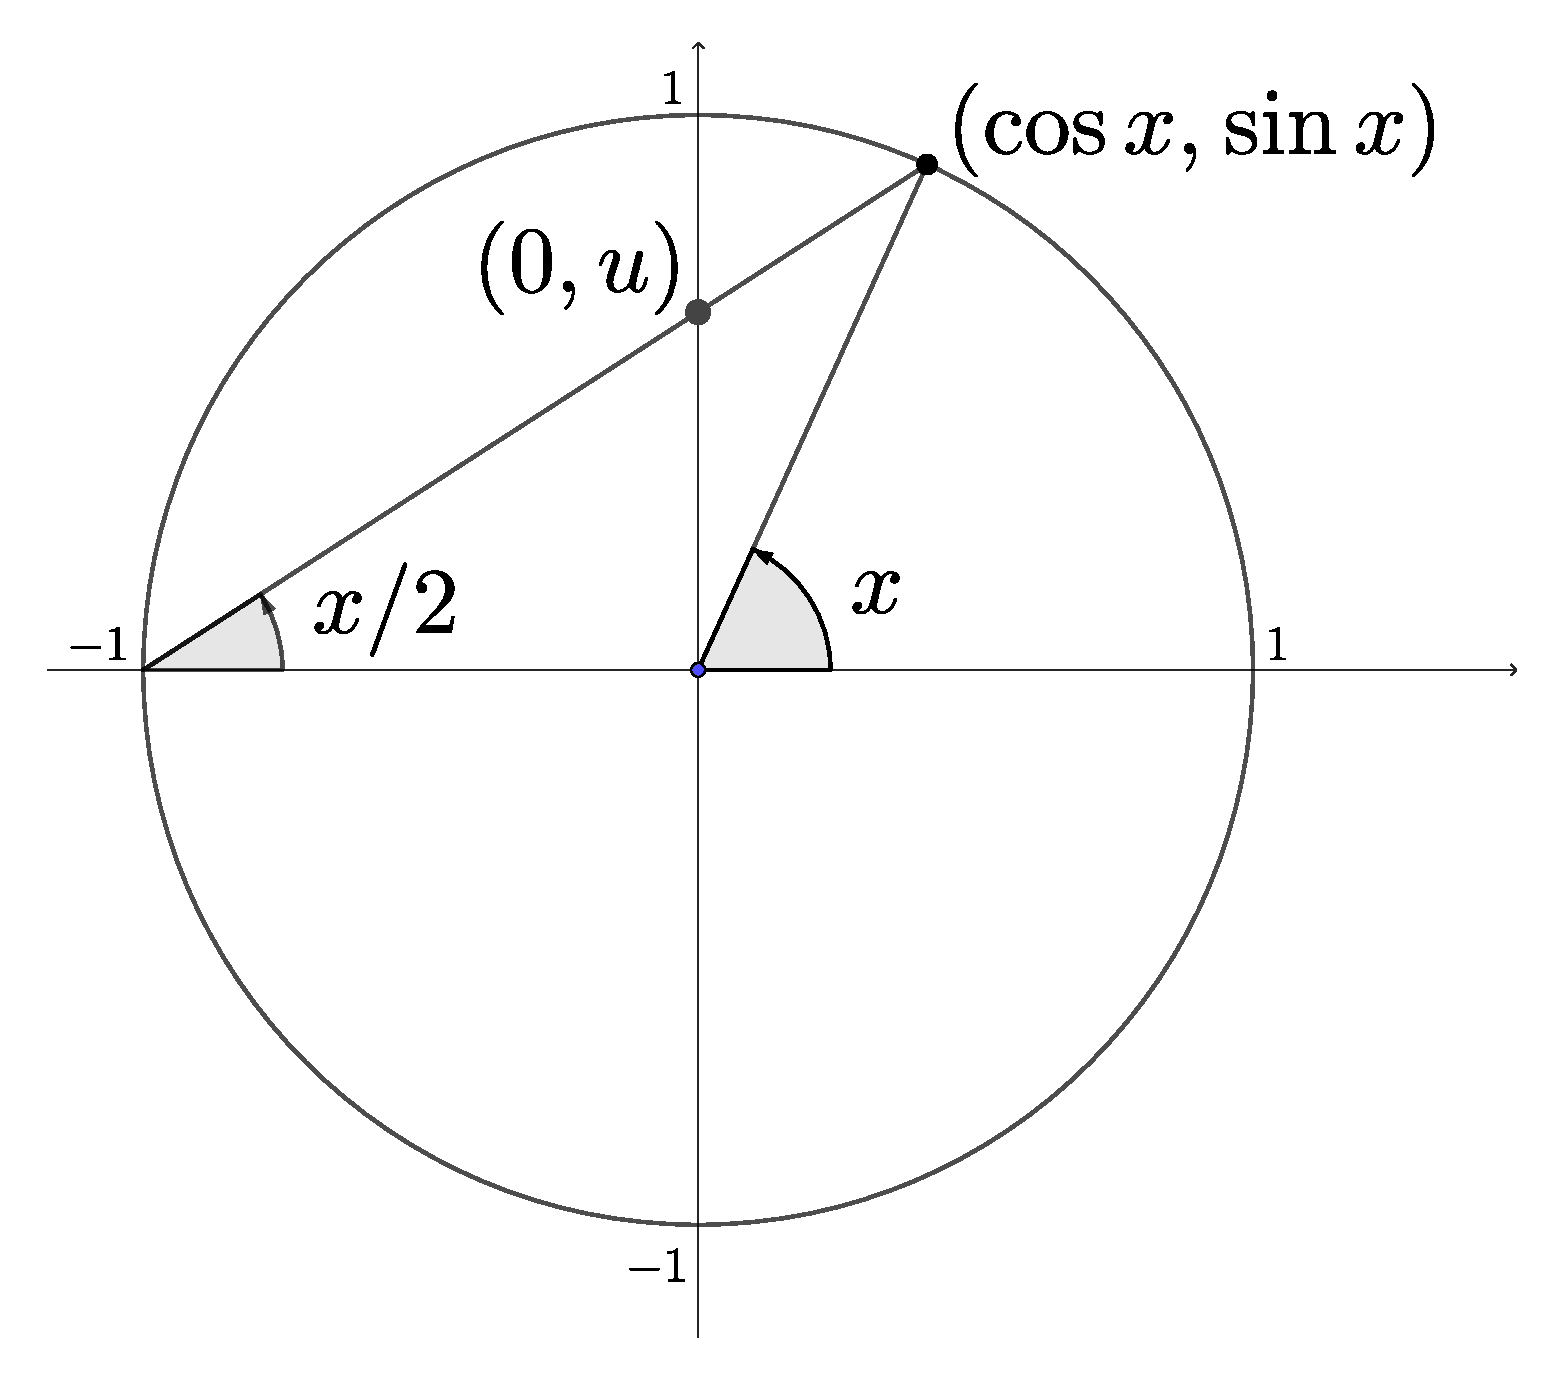
\includegraphics[height=7cm]{./pictures/03/u-tanx2.pdf}
\end{figure}

\newpage

前ページで紹介した「$\cos x$ と $\sin x$ と定数の四則演算だけで構成される関数」の中でもさらに
\begin{center}
  $\cos^2 x$ と $\sin^2 x$ と $\left( \sin x \right) \left(\cos x\right)$ と定数の四則演算だけで構成される関数
\end{center}
に関しては,変数変換 $\ds u=\tan x$ による置換積分で計算することもできる.例として
\[
  \int_{0}^{\pi/4} \frac{1+\cos^2x}{\sin^2 x + 3 \cos^2 x} \ dx
\]
を計算してみよう.さっそく $\ds u=\tan x$ とおく.このとき,
\[
  \cos^2 x = \frac{1}{1+\tan^2 x} = \frac{1}{1+u^2} \qquad \sin^2 x = 1- \cos^2 x = 1- \frac{1}{1+u^2} = \frac{u^2}{1+u^2}
\]
である.ちなみに,今回は使わないが
\[
  \left( \sin x \right) \left(\cos x\right) = \frac{\sin x}{\cos x}~ \cos^2 x = \left( \tan x \right)\left( \cos^2 x\right)
  = \frac{u}{1+u^2}
\]
である.さらに,
\[
  \frac{du}{dx} = 1+\tan^2 x = 1+u^2 \quad \text{ より } \quad 1 = \frac{1}{1+u^2} \frac{du}{dx} 
\]
である.また,積分範囲は $
\begin{array}{c|ccc}
  x & 0 & \to & \pi/4\\ \hline
  u & 0 & \to & 1
\end{array}
$ と変換されるので,この積分は次のように計算できる.
\[
  \begin{aligned}
    \int_{0}^{\pi/4} \frac{1+\cos^2x}{\sin^2 x + 3 \cos^2 x} \ dx
    &= \int_{0}^{\pi/4} \frac{1+ \frac{1}{1+u^2}}{ \frac{u^2}{1+u^2} + \frac{3}{1+u^2}} \frac{1}{1+u^2}~ \frac{du}{dx} \ dx
      = \int_{0}^{1} \frac{u^2+2}{(u^2+1)(u^2+3)} \ du\\[2ex]
    &= \int_{0}^{1}\left(\frac{\frac{1}{2}}{u^2+1} + \frac{\frac{1}{2}}{u^2+3}\right) \ dx 
      = \frac{1}{2}\left( \Big[ \tan^{-1}u \Big]_{0}^{1} + \left[ \frac{1}{\sqrt{3}}
      \tan^{-1}\frac{u}{\sqrt{3}}\right]_{0}^{1}\right)\\[2ex]
    &=\frac{\pi}{8}  + \frac{\sqrt{3}~\pi}{36}
  \end{aligned}
\]

なお,この変数変換における $u$ と $x$ の関係には下図のような意味づけができる.
\begin{figure}[h]
  \centering
  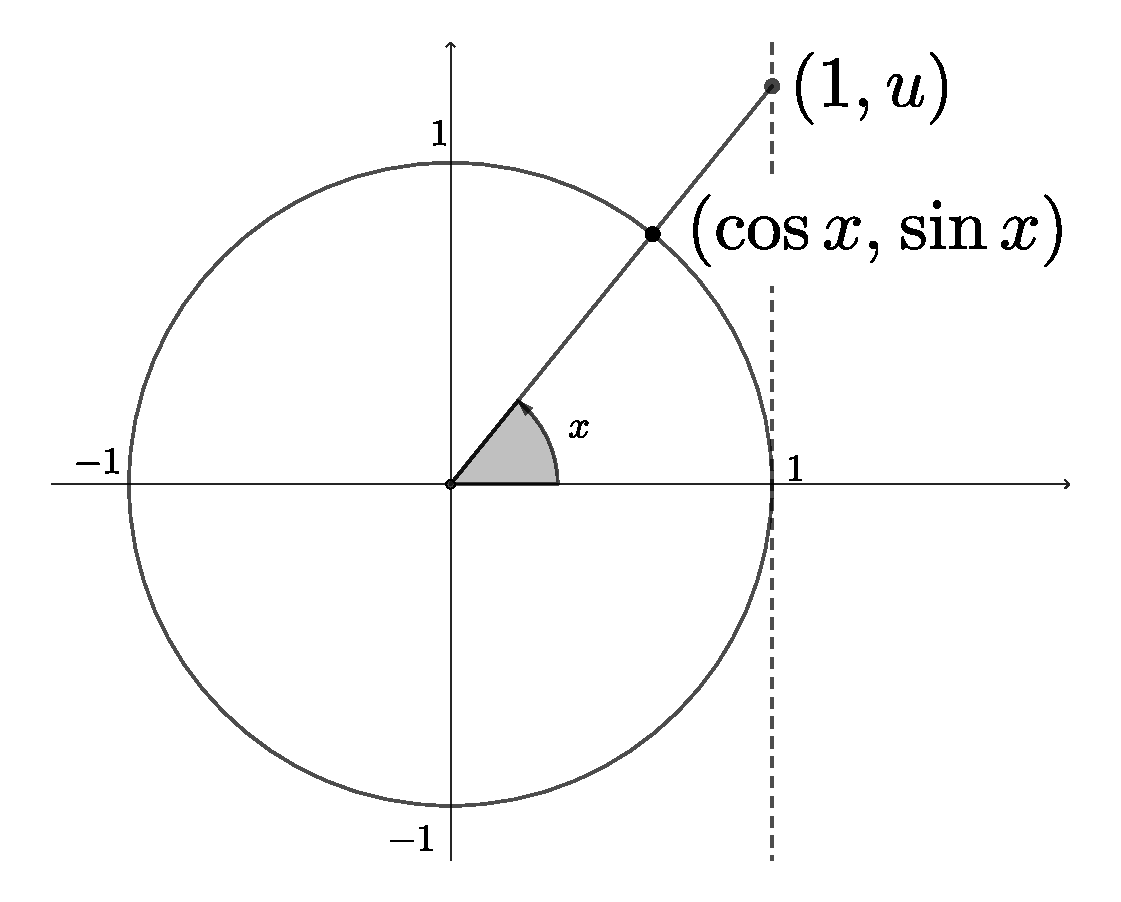
\includegraphics[height=6.5cm]{./pictures/03/u-tanx.pdf}
\end{figure}

\newpage

さらに特別な場合として,$\left(\sin^m x\right)\left(\cos^nx\right)$ の
積分を考える.例として,以下の $m=2,n=3$ の場合を計算してみるが,$m,n$
の少なくとも一方が奇数なら同様に計算できる.
  \[
    \int_{0}^{\pi/2} \left( \sin^2 x\right) \left( \cos^3 x \right) \ dx
  \]
  これも $\ds u=\tan\frac{x}{2}$ による置換積分で分数関数の積分に帰着できるが,かなり面倒な計算になる.そこで
  \[
    \left( \sin^2 x\right) \left( \cos^3 x\right) = \left( \sin^2 x\right) \left(\cos^2 x\right) \cos x
    = \left( \sin^2 x\right)\left(1-\sin^2 x\right) \cos x
  \]
  と変形してみると,$u=\sin x$ による置換積分がうまくいきそうなことに気
  がつける.実際,$\ds \frac{du}{dx} = \cos x$ であり,積分範囲が
  \[
    \begin{array}{c|ccc}
      x & 0 & \to & \pi/2\\ \hline
      u & 0 & \to & 1
    \end{array}
  \]
  と変換されるので,以下のように割と簡単に計算できてしまう.
  \[
    \int_{0}^{\pi/2} \left( \sin^2 x\right) \left( \cos^3 x\right) \ dx
    = \int_{0}^{1} u^2 \left( 1-u^2\right) \ du = \left[ \frac{u^3}{3} - \frac{u^5}{5}\right]_{0}^{1} = \frac{2}{15}
  \]\\

  続いて,以下の $m=2,n=4$ の場合を計算してみる.$m,n$ の両方が偶数なら同様に計算できる.
  \[
    \int_{0}^{\pi/2} \left( \sin^2 x\right) \left( \cos^4 x\right) \ dx
  \]
  これも $\ds u=\tan\frac{x}{2}$ や $u=\tan x$ による置換積分で分数関数
  の積分に帰着はできるが,まず
  \[
    \left( \sin^2 x\right) \left( \cos^4 x\right) = \left( 1-\cos^2 x\right) \cos^4 x  = \cos^4x - \cos^6 x
  \]
  と変形してみる.ここで半角の公式から
  \[
    \begin{aligned}
      \cos^4 x &= \left( \cos^2 x\right)^2 =
      \left(\frac{1+\cos(2x)}{2}\right)^2 = \frac{1+2\cos(2x) +
        \cos^2(2x)}{4}
      = \frac{1+2\cos(2x) + \frac{1+\cos(4x)}{2}}{4}\\
      &= \frac{3}{8} + \frac{\cos (2x)}{2} + \frac{\cos (4x)}{8}\\ \\
      \cos^6 x &= \left( \cos^2 x\right)^3 = \left(
        \frac{1+\cos(2x)}{2}\right)^3 = \frac{1+3\cos(2x) +
        3\cos^2(2x) + \cos^3(2x)}{8}\\
      &= \frac{1+3\cos(2x) + 3 \frac{1+\cos(4x)}{2}}{8} + \frac{\cos^3(2x)}{8}
      = \frac{5}{16} + \frac{3}{8}\cos(2x) + \frac{3}{16}\cos(4x) + \frac{\cos^3(2x)}{8}
    \end{aligned}
  \]
  なので,この積分は以下のように計算できる.
  \[
    \begin{aligned}
      \int_{0}^{\pi/2} \left(\sin^2 x\right)\left(\cos^4x\right) \ dx
      &= \int_{0}^{\pi/2}\left( \frac{1}{16} + \frac{\cos(2x)}{8} - \frac{\cos(4x)}{16} - \frac{\cos^3(2x)}{8}\right) \ dx\\
      &= \left[\frac{x}{16} + \frac{\sin(2x)}{16} - \frac{\sin(4x)}{64}\right]_{0}^{\pi/2}
      - \frac{1}{8}\int_{0}^{\pi/2}\cos^3(2x) \ dx\\
      & = \frac{\pi}{32} - \frac{1}{8}\int_{0}^{\pi/2}\cos^3(2x) \ dx = \frac{\pi}{32}
    \end{aligned}
  \]
  最後に残った積分は,$\cos^3(2x) = \left(1-\sin^2(2x)\right)
  \cos(2x)$ と変形できるので $u=\sin(2x)$ による置換積分で計算できる.
 
\end{document}
